\documentclass[11pt]{article}
\usepackage{fontspec,luatexja-fontspec}
\setmainjfont{HaranoAjiMincho-Regular.otf}
\usepackage[letterpaper,margin=1.03in]{geometry}
\usepackage{amsmath,amssymb,amsthm,mathtools,bm}
\usepackage{graphicx,booktabs,enumitem,float,tabularx}
\usepackage[numbers,sort&compress]{natbib}
\usepackage{placeins}
\usepackage[colorlinks=true,citecolor=blue!55!black,linkcolor=blue!50!black,urlcolor=blue!55!black]{hyperref}
\usepackage{xcolor}
\usepackage{caption}
\captionsetup{font=small,labelfont=bf}
\setlength{\parindent}{1.2em}
\setlength{\parskip}{0.16em}
\setlength{\emergencystretch}{1em}
\numberwithin{equation}{section}
\newtheorem{theorem}{定理}[section]
\newtheorem{proposition}[theorem]{命題}
\newtheorem{corollary}[theorem]{系}
\newtheorem{lemma}[theorem]{補題}
\theoremstyle{definition}
\newtheorem{definition}[theorem]{定義}
\newtheorem{assumption}[theorem]{仮定}
\theoremstyle{remark}
\newtheorem{remark}[theorem]{注意}
\hypersetup{pdftitle={ニュースなしに市場はいつ暴落しうるか？},pdfauthor={Siyuan Ye},pdfsubject={システミック・ドローダウンの到達可能性に関するモデル固有の理論}}
\newcommand{\R}{\mathbb{R}}
\newcommand{\Cris}{\mathcal{C}}
\newcommand{\calK}{\mathcal{K}}
\newcommand{\calA}{\mathcal{A}}
\newcommand{\dd}{\,\mathrm{d}}
\newcommand{\one}{\mathbf{1}}
\newcommand{\pos}[1]{[#1]_+}
\newcommand{\Law}{\mathcal{L}}
\newcommand{\totv}{\operatorname{TV}}
\title{\textbf{ニュースなしに市場はいつ暴落しうるか？}}
\author{Siyuan Ye\\{\small 独立研究者}}
\date{2026年10月}
\renewcommand{\proofname}{証明}
\renewcommand{\abstractname}{要旨}
\renewcommand{\figurename}{図}
\renewcommand{\tablename}{表}
\begin{document}
\maketitle
{\small 訳文声明：数学上の権威は英語原稿である。基準版 e5339a47f29ccb669d1f228ca930a1c1146200bf、2026-10-15。著者による訳文審査は未完了である。}\par
\vspace{-0.95em}
\begin{abstract}\noindent
ファンダメンタルズが固定され、売買代金のペア決済を行う回復力のある$N$資産市場において、応答弾力性$e(S)=Sg'(S)/g(S)\ge2$はすべての正のシステミック・ドローダウンを排除し、$e(S)\ge1$は全資産の同時下落を排除することを証明する。証明は、売買代金の移転と座標変位を等しくするよう一意に規格化された応答適合型一般化価格座標$\Phi(S)=\int_F^S u/g(u)\,\mathrm{d}u$を用いる。これにより加法的な取引保存則と、回復による安定性障壁が明らかになる。共通の関数族$g_p(S)=\eta(S/F)^p$において、$p=2,1,0$はそれぞれ排除、在庫によって制限された一部資産の損失、およびパルスを許した場合に一様な有限売買代金・在庫の下で任意に深刻となる一部資産の対数損失を与える。必要な売買代金および株数在庫の下界を示す。株当たり一定インパクトと有界な総売買執行速度の下で、小速度における最大システミック損失は二次のオーダーであり、このオーダーを達成する連続構成を与える。ローリング日次値幅は各セッションを制約するが、複数日の損失を必ずしも排除しない。計算機支援による十資産の経路では、九資産が連続する二セッションで下限終値に達し、すべての累積売買代金フローがゼロとなり、$0.020$を超えるシステミック対数損失を達成する。本例で必要な総執行速度上限は$0.044<\bar v_*<0.285$を満たす。
\end{abstract}
\noindent\textbf{キーワード：} 市場暴落；価格インパクト；市場の回復力；システミック・ドローダウン；到達可能性；執行制約。\par
\noindent\textbf{MSC 2020:} 91G15, 91G45, 93B03, 65G30, 91G80.

\section{序論}\label{sec:intro}
大幅な市場下落は必ずしも悪いニュースに続いて生じるわけではない。取引自体が限界価格を変え、市場の回復力がその変位の残存量を決める。したがって基本的かつ重要な問いは、ファンダメンタルズが不変の市場が、自らの決済規則に従う取引によって広範な同時損失へ押し込まれうるかである。本研究の問いは、均衡がどのように暴落を選択するかより限定的である。すなわち、どのシステミック損失状態が到達可能で、その到達にどのような執行資源が必要かを問う。

既存研究は、ニュースなしの価格変動を異なる市場機構から説明する。Gennotte and Leland~\citep{GennotteLeland1990}は動的ヘッジと推論を分析し、Romer~\citep{Romer1993}は外部ニュースを伴わない取引を通じた情報開示を研究する。Huang and Wang~\citep{HuangWang2009}は非同期の取引需要が内生的注文不均衡を生むことを示し、Cespa and Foucault~\citep{CespaFoucault2014}は資産間流動性のフィードバックを記述する。関連する多資産設定で、Cont and Wagalath~\citep{ContWagalath2013}は窮迫売却による内生的な収益依存を導く。これらのモデルは流動性に起因する不安定性の重要性を示す。本研究は、所与の執行則、価格の回復ダイナミクス、および各資産の終端累積売買代金フローのゼロ条件と両立する同時終端損失は何か、という補完的な数学的問いを扱う。

Kyle~\citep{Kyle1985}の均衡価格応答は古典的な出発点の一つである。価格インパクトと回復のモデルは、この問いを定量化する道具を与える。Obizhaeva and Wang~\citep{ObizhaevaWang2013}とAlfonsi and Schied~\citep{AlfonsiSchied2010}は回復力のある流動性下の執行を特徴づけ、Gatheral~\citep{Gatheral2010}、Alfonsi, Schied, and Slynko~\citep{AlfonsiSchiedSlynko2012}、Huberman and Stanzl~\citep{HubermanStanzl2004}は取引費用と価格操作の基準から制約を導く。多変量一時的インパクトはAlfonsi, Kl\"ock, and Schied~\citep{AlfonsiKlockSchied2016}が分析し、Cordoni and Lillo~\citep{CordoniLillo2024}は複数主体・多資産インパクトゲームの均衡不安定性を研究する。Kyle and Obizhaeva~\citep{KyleObizhaeva2023}は市場ミクロ構造の不変性を通じて、大口取引と執行速度を観測された暴落に結びつける。本研究はこれらの機構を動機として、指定した決済プロトコル下で実行可能なシステミック損失状態を特徴づけ、その状態への経路に課される売買代金、在庫、速度、値幅の制約を定量化する。

本研究は現金を用いないリスク資産再配分プールを扱う。各売却執行は等額のリスク資産購入と対になり、全資産の終端符号付き売買代金フローがゼロとなる。価格は固定基準$F$へ回復し、約定株数は正の応答関数$g(S)$を介して限界価格を動かす。鍵となるのは応答適合型座標で価格を測ることであり、通常は非線形な売買代金の効果が加法的になる。ペア取引は座標の和を保存し、回復力は取引間でその和を変える。座標の曲率は排除障壁を与え、共通制約下の三つの応答領域を統一する。次に、執行資源と取引所制約を課した後も、構造的に許される損失のうち何が達成可能かを問う。

有界な総売買執行速度と日次値幅の下で、到達可能性には許容終端価格以上のものが必要となる。多数の資産が下落すると、他の資産は対応する売買代金を受け入れなければならないが、その価格と執行速度も制約される。さらに、その上昇は危機基準に入る平均損失を相殺しうる。必要速度と部分集合間容量の下界を導き、十資産中九資産が仮想下限で反復して引ける明示的な二日間の経路を検証する。その結果は、明記した経路制約をすべて満たす認証付き複数日システミック・ドローダウン構成例である。これは必要資源不等式に対して明示的な存在例を与える。

分析は構造障壁から必要資源へ、さらに執行制約から同時実行可能性の認証へ進む。まず主要結果を述べ、その後に共通の市場定義と証明を示す。

\begin{theorem}[主要結果の概略]\label{thm:informal}
第\ref{sec:model}節で定義する回復力のある売買代金ペア決済市場では、以下が成り立つ。
\begin{enumerate}[label=\textup{(\roman*)},leftmargin= 2 em,itemsep= 0.12 em]
\item \emph{構造的排除。} 全許容価格で$e(S)=Sg'(S)/g(S)\ge2$なら、すべての対象範囲と時刻について$\Cris_\alpha(t)\le0$である。より弱い条件$e(S)\ge1$は全資産の同時下落を排除する。
\item \emph{到達可能性の領域。} $g_p(S)=\eta(S/F)^p$において、$p=2,1,0$はそれぞれ排除、在庫で制限された一部資産のドローダウン、および$k=\lceil\alpha N\rceil<N$で十分長い有限期間においてパルスを許せば固定された有限の売買代金・在庫上限下で任意に深刻な一部資産損失を生む。一定インパクトで$k=N$の場合、無制限の深度に代わり期間に依存する鋭い上界が得られる。
\item \emph{執行資源。} 一般の正の$g$について、必要な売買代金と株数在庫の明示的下界を得る。株当たり一定インパクトと有界な総売買執行速度の下で、小速度の危機上界は二次となり、そのオーダーは終端売買代金ゼロの連続構成で達成される。
\item \emph{複数日執行。} ローリング値幅はセッションごとの損失を制限し、速度制限と受入資産の容量は連続下限終値を制限する。計算機支援による二日間十資産経路はこれらの制約を満たし、九資産が反復下限終値を取り、$\Cris_{0.9}(T)>0.020$を与える。この例では$0.044<\bar v_*<0.285$である。
\end{enumerate}
\end{theorem}

共通の数学的道具は、次の\emph{応答適合型一般化価格座標}である。
\begin{equation}\label{eq:phi-intro}
\Phi(S)=\int_F^S\frac{u}{g(u)}\dd u.
\end{equation}
この座標では、一単位の売買代金が価格状態を一単位変位させる。ペア取引中の加法的保存則と取引間の復元ドリフトによって、構造障壁、資源、複数日執行の結果が結びつく。

\section{市場：仮定、執行、価格ダイナミクス}\label{sec:micro}\label{sec:model}
各売却執行に等額購入が対応するリスク資産再配分部分市場を定める。決済と価格応答は別個の仮定であり、前者はフローを制約し、後者は誘発される価格運動を決める。以下のすべての定理は同じ市場定義を用いる。

\begin{assumption}[回復力のある売買代金ペア決済市場]\label{asmp:model}
$N\ge2$資産と有限期間$[0,T]$を固定する。以下が共同して許容市場を定義する。
\begin{enumerate}[label=\textup{(M\arabic*)},leftmargin= 2.9 em,itemsep= 0.20 em]
\item \textbf{正の価格と座標。} 各取引価格$S_i(t)$は厳密に正で、初期値は$S_i(0)=F>0$である。狭義単調増加な$C^1$座標$q_i=\phi_i(S_i)$は価格優先を保存する。分析対象は決定論的な許容執行経路である。
\item \textbf{取引と執行の会計。} 約定株数変化は符号付き量$\dd\theta_i$である。符号なし出来高はその絶対増分を数え、両当事者を二重計上しない。執行は限界価格決済$\dd X_i=S_i\dd\theta_i$に従う。マッチングは注文板を条件として価格優先を用いる。有効価格応答は別途課す正で局所的に$C^2$の関数$g(S)$で、$\dd S_i|_{\rm trade}=g(S_i)\dd\theta_i$を満たす。
\item \textbf{ファンダメンタルズのニュース不在と回復力。} 基準$F$は固定される。取引間では価格は$F$へ、共通の一定速度$\rho>0$で回復する。執行がなければ$\dot S_i=-\rho(S_i-F)$である。応答関数$g$と$\rho$は\emph{モデル入力}であり、価格優先の帰結ではない。
\item \textbf{売買代金ペア決済ネットワーク。} 各許容取引は出発資産から到着資産へ等額の売買代金を移す。すなわち$\dd\bm X=B\dd\bm z$であり、$B$は完全双方向グラフの向き付き接続行列、$\dd\bm z\ge0$、$\one^\top B=0$である。これは選択したペア再配分部分市場を表す。積極的注文圧力がゼロ和であることは、すべての現実市場に関する一般的事実ではない。
\item \textbf{許容制御と終端ゼロ条件。} 経路は区分連続で執行変動が有限であり、限界価格決済による有限個の瞬間パルスを許す。全価格は正を保ち、必要な売却在庫は空売りなしに利用可能とする。終端比較では各資産に$X_i(T)=0$を課し、$\theta_i(T)=\theta_i(0)$を課すのではない。資源上限を主張する場合、市場間で同じ総ペア売買代金と資産別初期株数制限を課す。
\end{enumerate}
\end{assumption}



\paragraph{売買代金元帳をゼロにする理由。}
(M4)の完全双方向グラフは理想化したポートフォリオ切替プール、または約定売却代金が直ちに他のリスク資産の購入に使われる現金なし再配分枠を表す。これは通常の取引所全体の注文フローの恒等式ではなく、一般の株式市場では現金勘定や追加の取引相手が代金を吸収しうる。より強い終端条件$X_i(T)=\int_0^T S_i\,\dd\theta_i=0$を課すのは、全資産の一次純売買代金再配分が相殺された後の残存価格変位を調べるためである。これは研究上の規格化であり、通常の往復取引の定義ではない。株数中立の往復取引は$\theta_i(T)=\theta_i(0)$を課し、両制約の含意は異なる。特に後述の\eqref{eq:cost}から、終端変位または正の回復散逸を伴う売買代金ゼロ条件は、初期に利用可能な株数在庫の消費を必要とする。すなわち$F[\theta_i(0)-\theta_i(T)]=E(S_i(T))+\rho\int_0^T(S_i-F)^2/g(S_i)\,\dd t$である。終端売買代金ゼロ条件は株数を元に戻さない。この区別は障壁結果に不可欠である。

\paragraph{有限変動経路と限界価格決済パルス。}
絶対連続制御では微分記法は通常の意味である。跳躍では左端点または右端点Stieltjes積$S_i\Delta\theta_i$を\emph{用いない}。物理時間を固定し、各有向辺$e:i\to j$について売買代金量$z>0$を、指定したイベント内パラメータ$a\in[0,z]$に沿って執行する。
\begin{equation}\label{eq:pulse-flow}
\frac{\dd \widetilde S_i}{\dd a}=-\frac{g(\widetilde S_i)}{\widetilde S_i},\quad
\frac{\dd \widetilde S_j}{\dd a}=\frac{g(\widetilde S_j)}{\widetilde S_j},\quad
\frac{\dd\widetilde\theta_i}{\dd a}=-\frac{1}{\widetilde S_i},\quad
\frac{\dd\widetilde\theta_j}{\dd a}=\frac{1}{\widetilde S_j}.
\end{equation}
結果の端点フローは$\Delta X_i=-z$、$\Delta X_j=z$、および$\Delta\Phi(S_i)=-z$、$\Delta\Phi(S_j)=z$を満たす。同値に、単一株数インパルスは$\dd\widetilde S/\dd\xi=g(\widetilde S)$を解き、その応答軌道に沿って$\int\widetilde S\,\dd\xi$を積分して評価する。したがって跳躍は通常の連鎖律を保存する\emph{フロー補完型}（Marcus型）の更新である。異なる辺の有限パルスは指定順に処理する。全中間価格が厳密に正である間だけパルスは許容される。以下のすべての跳躍表現はこの規則で解釈する。

\paragraph{条件付きマッチング写像から有効応答へ。} 凍結注文板$\mathcal B$を固定し、その株数厚み密度$\rho_S(S;\mathcal B)$は局所的に正で連続とする。符号付き限界株数$\dd\theta$の一方向スイープは次の局所関係に従う。
\begin{equation}\label{eq:frozen-depth}
\dd\theta=\rho_S(S;\mathcal B)\dd S,
\qquad \rho_q(q;\mathcal B)\dd q=\rho_S(S;\mathcal B)\dd S.
\end{equation}
厳密な離散版は注文板の累積厚みの一般化逆関数を用いる。連続近似では$q=\phi(S)$の変更はJacobianを通じて密度の数値を変えるが、マッチング優先順位を変えない。この関係は限界約定価格を指す。動的仲値、注文補充、および資産間クロスインパクトは座標変換から導かれない。代わりに仮定(M2)は、以下で$g(S)=1/\rho_S^{\rm eff}(S)$を状態依存の\emph{有効}応答として選ぶ。

\paragraph{得られる$N$資産方程式。} 完全な市場仕様の下で、価格水準の法則は次式となる。
\begin{equation}\label{eq:level-dynamics}
\boxed{\dd S_i(t)=-\rho\big(S_i(t)-F\big)\dd t+g(S_i(t))\dd\theta_i(t),\qquad \dd X_i=S_i\dd\theta_i.}
\end{equation}
狭義単調な一般化座標$q_i=\log(S_i/F)$を選ぶ。ペア売買代金への変換は次式を与える。
\begin{equation}\label{eq:log-impact}
\dd q_i\big|_{\rm trade}=\frac{g(S_i)}{S_i^2}\dd X_i.
\end{equation}
この変換、取引のペア化、および回復力を組み合わせると、多資産系全体は次式となる。
\begin{equation}\label{eq:master}
\boxed{\dd\bm q=-\rho(\one-e^{-\bm q})\dd t+D(\bm q)B\dd\bm z,\qquad
D_{ii}(\bm q)=\frac{g(Fe^{q_i})}{F^2e^{2q_i}}.}
\end{equation}
指数関数は成分ごとに作用する。この対数座標は損失測定に便利だが、売買代金にはより単純な応答適合型座標がある。$y_i=\Phi(S_i)$とし、$\Phi$は\eqref{eq:phi-intro}で定める。この座標は狭義単調増加で$\Phi(F)=0$を満たす。さらに微分可能座標$\psi$を$\psi(F)=0$で規格化すると、各限界取引で$\dd\psi(S)|_{\rm trade}=\dd X$を要求することは$\psi'(S)g(S)=S$を強制し、$\psi=\Phi$を一意に選ぶ。復元応答を次式で定める。
\[
\mathcal R(y)=\frac{S(S-F)}{g(S)},\qquad S=\Phi^{-1}(y).
\]
多資産市場全体は次の\emph{取引規格化形}となる。
\begin{equation}\label{eq:normal-form}
\boxed{\dd\bm y=B\dd\bm z-\rho\mathcal R(\bm y)\dd t,\qquad\one^\top B=0,}
\end{equation}
ここで$\mathcal R$は成分ごとに作用し、執行則はフロー補完パルスにも適用される。取引は加法的なゼロ和入力であり、非線形な価格状態依存はすべて復元項と逆写像$S=\Phi^{-1}(y)$へ移る。変換後の状態空間は$\mathcal J^N$で、$\mathcal J=\Phi((0,\infty))$である。$g_p(S)=\eta(S/F)^p$について、値域は$(-F^2/[\eta(2-p)],\infty)$（$p<2$の場合）、$\mathbb R$（$p=2$の場合）、$(-\infty,F^2/[\eta(p-2)])$（$p>2$の場合）となる。したがって加法的取引入力によって厳密な価格正値性や執行制約は消えない。座標変換は価格状態の到達可能性を変えない。$\rho=0$では一般化座標の取引和は厳密に保存される。

\begin{definition}[終端システミック・ドローダウン]\label{def:crash}
$L_i(T)=\log[F/S_i(T)]$、$\overline L(T)=N^{-1}\sum_i L_i(T)$とする。$k$番目に大きい損失（ここで$k=\lceil\alpha N\rceil$）を$Q_\alpha(T)$と書く。次を定義する。
\begin{equation}\label{eq:crash}
\boxed{\Cris_\alpha(T)=\min\{\overline L(T),Q_\alpha(T)\}.}
\end{equation}
$\delta>0$について、$\Cris_\alpha(T)\ge\delta$のとき\emph{終端危機}が発生する。すなわち平均損失と少なくとも$k$個の個別損失がそれぞれ$\delta$に達する必要がある。目標は価格応答関数と独立に選ぶ。
\end{definition}

離散的対象範囲の規則は重要である。$N=3$の場合、$\alpha=0.9$は$k=3$を意味し、三資産すべての下落を要求する。一般に$k=N$と$k<N$の違いは補償資産が存在するかを決める。同じ区別はまずA/B/C分類に現れ、その後、複数日の資産間容量不等式に現れる。初到達イベント$\tau_{\alpha,\delta}=\inf\{t:\Cris_\alpha(t)\ge\delta\}$は売買代金ゼロ条件下の\emph{終端}危機と異なり、本研究は後者を扱う。

\begin{definition}[売買代金、株数在庫、終端臨界予算]\label{def:budget}
許容経路$\gamma$について、次を定める。
\begin{equation}\label{eq:resource}
M(\gamma)=\sum_e\int_0^T\dd z_e,\qquad
H_i^-(\gamma)=\int_0^T\big(-\dd\theta_i\big)_+.
\end{equation}
許容初期在庫$H_i$と終端累積売買代金フローのゼロ条件の下で、次を定義する。
\begin{equation}\label{eq:minbudget}
M_*^{\rm end}=\inf\{M(\gamma): X_i(T)=0\ \forall i,\ \Cris_\alpha(T)\ge\delta,\ \gamma\text{ admissible}\},
\end{equation}
ここで$\inf\varnothing=+\infty$とする。ペア売買代金移転は二資産の元帳に反対符号で現れるが、$M$では一回だけ数える。
\end{definition}

\paragraph{利益を生む往復取引がないという性質の正確な意味。} 次を定義する。
\begin{equation}\label{eq:E}
E(S)=\int_F^S\frac{u-F}{g(u)}\dd u\ge0.
\end{equation}
$F$から始まる任意の許容経路について、執行費用恒等式は次式である。
\begin{equation}\label{eq:cost}
\boxed{\int_0^T S_i\dd\theta_i=F[\theta_i(T)-\theta_i(0)]+E(S_i(T))
+\rho\int_0^T\frac{(S_i-F)^2}{g(S_i)}\dd t.}
\end{equation}
したがって(M2)--(M3)の下で\emph{株数中立}の往復取引の執行費用は非負である。一方、本論文の終端条件$X_i(T)=0$は株数ではなく約定\emph{売買代金}をゼロにする。終端売買代金中立経路は初期在庫を消費しうる。付録\ref{app:accounting}でこの会計恒等式と許容制御への帰結を証明する。

\paragraph{株数中立取引との比較。}
終端売買代金条件と標準的な株数中立条件は交換可能ではない。例えば$g\equiv\eta$で、十分小さい$a>0$株を時刻$0$に購入し、$a$株を時刻$T$に売却した単一資産は$\theta(T)=\theta(0)$だが、終端価格は$S(T)=F-\eta a(1-e^{-\rho T})<F$となる。その純売買代金はゼロではなく、\eqref{eq:cost}の正の費用は現金勘定を通じて支払われる。逆に(M4)の下で、全資産について終端売買代金中立と\emph{同時に}株数中立を要求すると$\sum_i[E(S_i(T))+\rho\int_0^T(S_i-F)^2/g(S_i)\,\dd t]=0$を強制する。したがって両ゼロ条件の下では正の時間にわたる散逸的価格変動は起こりえない。売買代金中立プロトコルは、標準的な株数往復執行と異なる経済的問いを意図的に抽出する。

\section{市場暴落の構造的障壁}\label{sec:barriers}
標準形\eqref{eq:normal-form}は取引中に保存されるスカラーを与える。$H(\bm S)=\one^\top\bm y=\sum_i\Phi(S_i)$と書く。資産について和を取ると、すべての対応売買代金移転が相殺され、回復だけが残る。
\begin{equation}\label{eq:potential-law}
\boxed{\dd H=-\rho\sum_{i=1}^N\mathcal R(y_i)\dd t
=-\rho\sum_{i=1}^N\frac{S_i(S_i-F)}{g(S_i)}\dd t.}
\end{equation}
スカラー$H$は取引不変量であり、回復ダイナミクス全体の保存量ではない。回復ドリフトが$H$を危機境界の向こうへ運べるかは$\Phi$の曲率に依存する。
応答弾力性を次式で導入する。
\begin{equation}\label{eq:elasticity}
e(S)=\frac{Sg'(S)}{g(S)}.
\end{equation}
$\Phi$および$G(x)=\Phi(Fe^x)$の導関数は次式である。
\begin{equation}\label{eq:curvature}
\Phi''(S)=\frac{1-e(S)}{g(S)},\qquad
G''(x)=\frac{S^2}{g(S)}\,[2-e(S)],\quad S=Fe^x.
\end{equation}
二つの曲率の区別はシステミック損失の定義に対応する。\emph{全資産}が基準以下になることへの障壁は、\emph{平均}対数損失も含む本汎関数への障壁より弱い。したがって同じ座標から二種類の排除命題を得られる。


\begin{theorem}[全資産下落への障壁]\label{thm:barrier1}
許容経路で到達可能な全価格で$e(S)\ge1$なら、$S_i(t)<F$が全$i$について同時に成り立つことは、いかなる時刻$t$にも不可能である。特に$k=N$の正の危機は到達不可能である。
\end{theorem}
\begin{proof}
式\eqref{eq:curvature}により$\Phi$は凹となる。$S$における接線不等式は$\Phi(F)\le\Phi(S)+\Phi'(S)(F-S)$であり、したがって$(S-F)\Phi'(S)\le\Phi(S)$である。ゆえに\eqref{eq:potential-law}から取引間で$\dot H\ge-\rho H$を得る。パルスは$H$を保存する。$H(0)=0$なので比較により$H(t)\ge0$となる。すべての$S_i(t)<F$なら、狭義単調性と$\Phi(F)=0$から逆に$H(t)<0$となり、矛盾する。
\end{proof}

\begin{theorem}[任意対象範囲のシステミック危機への障壁]\label{thm:barrier2}
許容価格範囲で$e(S)\ge2$なら、すべての許容制御、$N\ge2$、$\alpha\in(0,1]$、および$t\in[0,T]$について次が成り立つ。
\begin{equation}\label{eq:no-crash}
\boxed{\Cris_\alpha(t)\le0.}
\end{equation}
したがって厳密に正のシステミック終端危機閾値には到達できない。
\end{theorem}
\begin{proof}
先の定理より$H(t)\ge0$である。\eqref{eq:curvature}の第二恒等式により$G(x)=\Phi(Fe^x)$は凹かつ狭義単調増加となる。Jensenの不等式から次を得る。
\[
0\le\frac{H(t)}N=\frac1N\sum_iG(q_i(t))
\le G\!\left(\frac1N\sum_iq_i(t)\right).
\]
$G(0)=0$で$G$は狭義単調増加なので$\sum_iq_i(t)\ge0$である。したがって平均損失$\overline L(t)=-N^{-1}\sum_iq_i(t)$は非正となり、定義\ref{def:crash}から\eqref{eq:no-crash}を得る。
\end{proof}

二つの定理は各仮定下でどの許容取引プログラムも到達できない状態を特定する。これらは大域的\emph{十分}条件であり、逆命題でも安定性の必要条件でもない。不等式が$F$近傍だけで成り立つなら、排除は全経路がそこにとどまる間だけ適用される。在庫、取引リンク、時間の制限はさらに障壁を生みうる。次の問いは構成的である。構造条件を緩めると到達集合は実際に変わるのか。A/B/C比較は、十分条件の不成立を暴落の証明と解釈せず、単一応答族内でこれに答える。

\section{共通制約下の三市場領域}\label{sec:regimes}
上の曲率条件は不可能なことを示すが、不等式が成立しないとき何が可能になるかは示さない。無関係なモデル間ではなく共通仮定下の違いを示すため、次の関数族の応答形状だけを変える。
\begin{equation}\label{eq:power}
 g_p(S)=\eta\left(\frac SF\right)^p,\qquad p\in\{2,1,0\},\quad \eta>0.
\end{equation}
三市場は同じ$N,T,F,\rho,\eta$、同じ初期価格と初期\emph{インパクト}、同じ売買代金ペア決済ネットワークを持ち、数値比較では同じ売買代金・在庫上限を用いる。相違は指数$p$だけである。対数・売買代金方程式\eqref{eq:master}では次式となる。
\begin{equation}\label{eq:powerd}
 D_{ii}^{(p)}(q_i)=\frac\eta{F^2}e^{(p-2)q_i},\qquad e(S)=p.
\end{equation}
同じ座標公式は各指数について明示的に積分できる。
\[
\Phi_p(S)=\begin{cases}
\displaystyle \frac{F^p}{\eta(2-p)}\big(S^{2-p}-F^{2-p}\big),&p\ne2,\\[4pt]
\displaystyle \frac{F^2}{\eta}\log(S/F),&p=2.
\end{cases}
\]
したがって$\sum_iS_i^2$、$\sum_iS_i$、$\sum_i\log S_i$に比例する量が、それぞれ$p=0,1,2$の場合にペア取引で保存される。取引間では回復がこれらを変化させる。図\ref{fig:response}は対応する売買代金当たり瞬間応答を示す。$F$以下では$p=0$の応答が売買代金取引を最も強く増幅する。

\begin{figure}[t]
\centering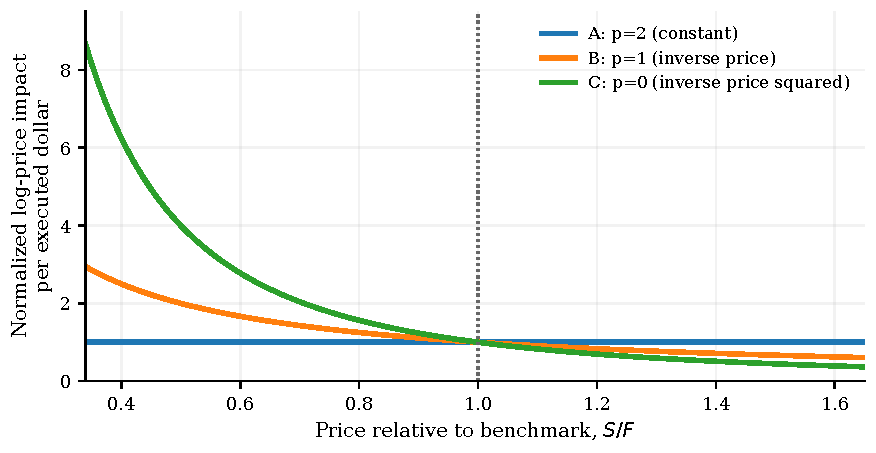
\includegraphics[width=0.82\linewidth]{../../paper/figures/response_regimes.pdf}
\caption{\textbf{単一応答族と三つの価格感応度。} 図はモデルが含意する瞬間的な\emph{売買代金当たり対数価格変化}を、共通初期値で規格化して示す。全曲線は$S=F$で一致する。これは理論比較であり、観測注文板への当てはめではない。}\label{fig:response}
\end{figure}

\begin{theorem}[A/B/C到達可能性領域]\label{thm:ABC}
$N\ge2$、$k=\lceil\alpha N\rceil<N$とする。同じモデルプロトコル下で\eqref{eq:power}の三市場を比較する。
\begin{enumerate}[label=\textup{(\Alph*)},leftmargin= 2 em,itemsep= 0.15 em]
\item \textbf{障壁市場（$p=2$）：} 全許容経路および全期間について$\Cris_\alpha(t)\le0$である。
\item \textbf{在庫制約市場（$p=1$）：} 正で十分小さい終端システミック・ドローダウンは到達可能である。各資産の初期在庫に固定した有限上限$H_0$があり空売りが禁止されるなら、終端危機深度は取引系列に依存しない上界を持つ。
\item \textbf{深刻損失到達市場（$p=0$）：} 固定したすべての$N\ge2$と$k<N$について、十分長い有限期間$T$と有限定数$M_0,H_0$が存在し、\emph{すべての}有限$\delta>0$に対し、$M\le M_0$、$H_i^-\le H_0$、$X_i(T)=0$を満たす許容正価格経路が$\Cris_\alpha(T)>\delta$を達成する。
\end{enumerate}
(C)の定数は$N,T,F,\rho,\eta$に依存しうるが、$\delta$には依存しない。$N\to\infty$で一様ではない。
\end{theorem}
\begin{proof}
(A)は定理\ref{thm:barrier2}から従う。(B)は命題\ref{prop:two-pulse}の二パルス構成と後述の在庫不等式\eqref{eq:inventoryb}から従う。(C)は付録\ref{app:severe}で構成的に示す。$N-1$の対象資産を任意にゼロへ近づけ、一資産をキャッシュフロー補償に用いる。制御は正の価格、完全にペア化された限界売買代金執行、回復時間の分割、および各$X_i$の終端ゼロ条件を用いる。明示的な売買代金・在庫上界は目標終端価格$\varepsilon\downarrow0$に依存しない。
\end{proof}

同じ売買代金・回復プロトコル下で、三つの応答関数は異なる到達状態幾何を生む。市場Aは大域的不変領域障壁を与える。市場Bは株数在庫が有限なら、非ゼロの一部資産損失が任意の大損失を許すとは限らないことを示す。市場Cは制御された深刻損失構成例を与える。(C)の$k<N$は不可欠で、少なくとも一資産が補償フローを担う必要がある。有限の総売買執行速度を課すと、これは存在要件にとどまらず明示的な\emph{容量}制約となる。

$p=1$の場合、\eqref{eq:E}の在庫ポテンシャルは次式となる。
\begin{equation}\label{eq:inventoryb}
E_1(Fe^{-L})=\frac{F^2}{\eta}\left(L+e^{-L}-1\right).
\end{equation}
\eqref{eq:cost}により、終端売買代金ゼロ条件と空売り禁止は$E_1(S_i(T))\le FH_0$を含意する。$L+e^{-L}-1\to\infty$が$L\to\infty$で成り立つので、固定有限在庫は必要な$k$資産の任意に深刻な損失を支えられない。一方$p=0$の場合、$E_0(S)=(S-F)^2/(2\eta)$は$S\downarrow0$でも有界である。これは(C)の構成を可能にするが、それだけで到達可能性を証明するものではない。

\begin{proposition}[局所全資産下落]\label{prop:three-pulse}
$g$が$C^3$級であることを$F$近傍で仮定し、$e(F)<1$とする。このとき、すべての$N\ge2$について、終端売買代金ゼロ、正価格、小振幅の三パルス制御で、\emph{全資産が}$S_i(T)<F$となるものが存在する。$c=g(F)/F^2$、$r=e^{-\rho T/2}$とし、ゼロ和インパルス方向$\bm u$を、すべての$u_i\ne0$を満たすように選ぶ。その損失は次を満たす。
\begin{equation}\label{eq:three-pulse}
L_i(T)=\frac{1-e(F)}2c^2h^2u_i^2r(1-r^2)+O(h^3)>0
\end{equation}
これは十分小さい$h>0$で成り立つ。
\end{proposition}
\begin{proof}
売買代金パルス$h\bm u$、$-(1+r)h\bm u$、$rh\bm u$を、それぞれ時刻$0,T/2,T$に与える。これらはペア売買代金均衡を満たし、全資産について和がゼロになる。座標$y=\Phi(S)$でのTaylor展開により\eqref{eq:three-pulse}を得る。詳細は付録\ref{app:local}に示す。
\end{proof}

\begin{proposition}[局所一部資産下落]\label{prop:two-pulse}
$k<N$、$e_0=e(F)<2$、$r=e^{-\rho T}<2-e_0$とする。少なくとも$k$個の正成分を持つゼロ和売買代金方向を選び、$h\bm u$を時刻$0$に、$-h\bm u$を時刻$T$に執行する。このとき$\Cris_\alpha(T)>0$が十分小さいすべての$h>0$で成り立ち、次式を得る。
\begin{equation}\label{eq:two-pulse}
\overline L(T)=\frac{c^2h^2}{2N}(1-r)(2-e_0-r)\sum_iu_i^2+O(h^3).
\end{equation}
\end{proposition}
\begin{proof}
個別損失は$L_i(T)=c(1-r)hu_i+O(h^2)$を満たす。$\sum_i u_i=0$なので平均では一次項が消える。\eqref{eq:two-pulse}の厳密に正の二次係数が結果を示す。付録\ref{app:local}を参照。
\end{proof}

次の二命題は分類の局所的側面を説明する。二パルス経路はより弱い弾力性閾値で一部資産損失を生み、追加の相殺段階を持つ三パルス経路は$e(F)<1$で\emph{全資産}の小下落を生みうる。両者は局所構成であり、市場Cの大域的深刻損失の議論を置き換えない。

\paragraph{共通予算による具体的比較。} $N=3$、$k=2$、$F=\eta=\rho=1$、$T=3$、共通売買代金上限$M_0=3$、資産別初期在庫上限$H_0=8.2$の場合、$p=2$市場はいかなる正の危機にも到達できない。$p=1$市場は小さい正の危機には到達できるが、閾値$\delta=10$には到達できない（条件を満たす各資産で$9$株超の売却が必要となる）。構成した$p=0$経路は$\Cris_{2/3}(T)\approx13.32$に達し、その売買代金は約$2.62$、資産別最大累積売却株数は$3.94$未満である。大きな$\delta$は有界・非有界の\emph{対数}損失を区別する厳密なストレステストとして選んだもので、代表的な実測暴落規模ではない。検証コードはソースに同梱される。


\begin{figure}[tbp]
\centering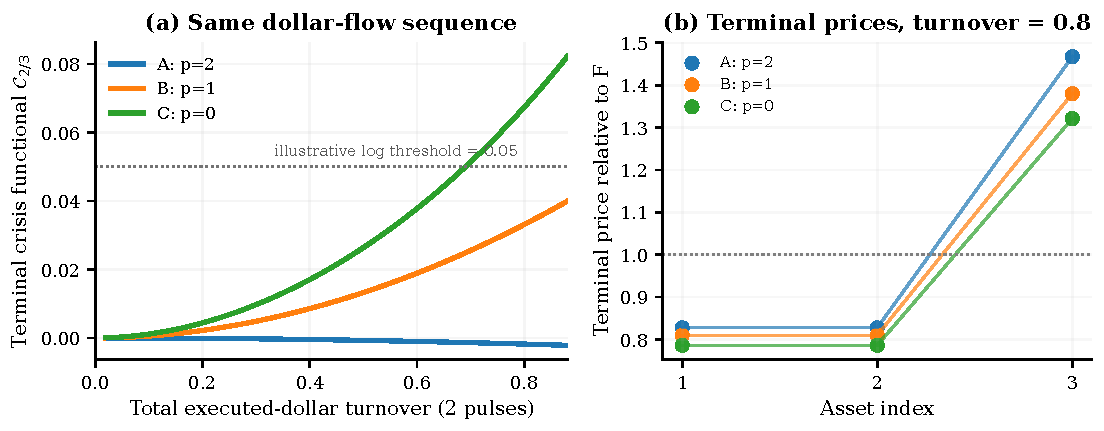
\includegraphics[width=0.98\linewidth]{../../paper/figures/abc_control_comparison.pdf}
\caption{\textbf{A/B/C応答関数に対する同一取引実験。} 終端で相殺する二つの売買代金パルスを、$N=3$、$k=2$、$F=\eta=\rho=1$、$T=3$の資産に与える。左：ペア売買代金増加に伴う\emph{終端}危機汎関数。右：同じ総売買代金$M=0.8$の下での終端価格。この局所例示は深刻暴落の存在構成とは別である。点線の閾値は例示であり、較正値ではない。}\label{fig:abcnum}
\end{figure}

\FloatBarrier
\subsection{全資産下落が必要な場合の鋭い境界}\label{sec:allcoverage}
市場Cは$k<N$に依存する。対象範囲条件が単なる技術的仮定ではないことを見るため、\emph{同じ一定インパクト応答}を保ち、目標を$k=N$に変える。この場合、他の$N-1$の終端損失を補償できる対象外資産が存在しない。固定執行予算を課す前から、任意深度の構成に代わって期間依存の厳密な上限が得られる。

\begin{theorem}[鋭い全資産期間閾値]\label{thm:critical}
仮定\ref{asmp:model}で$g(S)=\eta$、$k=N$とし、次を定義する。
\begin{equation}\label{eq:critical}
\boxed{\delta_{\mathrm{crit}}(N,T)=
\log\frac{\sqrt N}{1+(\sqrt N-1)e^{-\rho T}}.}
\end{equation}
すべての$\delta\in(0,\delta_{\mathrm{crit}}(N,T))$について、有限売買代金と十分大きな有限在庫により、ある許容終端売買代金ゼロ制御が$\Cris_1(T)\ge\delta$に達する。$\delta\ge\delta_{\mathrm{crit}}(N,T)$なら、そのような正価格経路は存在しない。したがって$\delta_{\mathrm{crit}}$は全資産共通対数ドローダウンの\emph{達成されない上限}である。
\end{theorem}
\begin{proof}[証明の概略]
$R(t)^2=\sum_iS_i(t)^2$とする。一定応答の下で任意のペア売買代金取引は$\dd R^2|_{\rm trade}=2\eta\sum_i\dd X_i=0$を満たす。取引間では次が成り立つ。
\[
\dot R=-\rho\left(R-F\frac{\sum_iS_i}{R}\right).
\]
正価格では$\sum_iS_i/R>1$であり、したがって$R(T)>F\{1+(\sqrt N-1)e^{-\rho T}\}$となる。各資産の終値が$Fe^{-\delta}$以下なら$R(T)\le F\sqrt Ne^{-\delta}$で、必要性が示される。十分性のため、価格ベクトルを一つの高い座標を持つ$N$個の正の球面方向へ回転させ、各資産に等しい回復重みを割り当てる。各方向変更はゼロ和のペア売買代金パルスで、回復段階のペア制御は方向を固定する。終端価格と回復積分が等しいこと、および$\sum_iX_i(T)=0$から、$X_i(T)=0$が全$i$について成り立つ。正の低座標をゼロへ近づけると連続的に上界へ近づく。完全な構成証明は付録\ref{app:sharp}に示す。
\end{proof}


\section{必要な取引量はどれほどか}\label{sec:budget}
ここまでの分類は市場が損失状態を許容するかに答えた。しかし参加者の利用可能資源で到達できるとは限らない。そこで価格状態幾何から第二の検査へ移る。指定した対象範囲と深度を達成するには、どれほどの売買代金と株数売却が必要か。以下の下界は一般の正応答で成り立ち、A/B/C到達可能性結果を補完する。

\begin{theorem}[執行資源の下界]\label{thm:resource}
許容終端経路が$\Cris_\alpha(T)\ge\delta>0$を満たすとする。$k=\lceil\alpha N\rceil$、$s=Fe^{-\delta}$と書く。$\Phi$に加え、単調な株数応答座標$\Psi(S)=\int_F^S\dd u/g(u)$を定義する。すると必要売買代金と総売却株数の下界は、それぞれ$s$までの座標距離となる。
\begin{equation}\label{eq:resource-lower}
\boxed{M\ge -k\Phi(s)=k\int_s^F\frac{u}{g(u)}\dd u,\qquad
\sum_iH_i^-\ge -k\Psi(s)=k\int_s^F\frac{\dd u}{g(u)}.}
\end{equation}
さらに$X_i(T)=0$で、空売りが許されず、条件を満たす資産の初期在庫が$H_i$を超えないなら、次が成り立つ。
\begin{equation}\label{eq:share-bound}
\boxed{\int_s^F\frac{F-u}{g(u)}\dd u\le FH_i.}
\end{equation}
これらは必要条件であって十分条件ではなく、必ずしも鋭くない。
\end{theorem}
\begin{proof}
終端条件を満たす資産の最終価格は高々$s<F$である。両変換座標は価格とともに増加し、回復は$F$におけるゼロ値へ向かう。したがって累積負売買代金変動と負株数変動はそれぞれ少なくとも$-\Phi(s)$、$-\Psi(s)$を必要とする。異なる$k$資産について和を取ると、各ペア執行は資産全体で売却としてちょうど一回数えられるため\eqref{eq:resource-lower}を得る。式\eqref{eq:share-bound}は、$X_i(T)=0$および$\theta_i(0)-\theta_i(T)\le H_i$を用いて\eqref{eq:cost}の非負右辺から従う。詳細な変動の議論は付録\ref{app:accounting}に示す。
\end{proof}

資源下界は二つの単調座標の幾何学的距離であり、最適取引日程ではない。取引方向、回復時間、受入資産の購買容量はさらに要件を課す。次にこれらの執行制約を扱う。

同じ市場の厚みを\emph{複製して}$N$を増やし、$\alpha,\delta$を固定すると、$k=\Theta(N)$となり、目標が到達可能なら\eqref{eq:resource-lower}は$M_*^{\rm end}=\Omega(N)$を含意する。これは現実の取引所に普遍的な時価総額調整則ではない。この実験で$N$を増やすことは集計市場厚みも増やすからである。

低価格積分は異なる資源不足を区別する。
\begin{equation}\label{eq:lowprice}
\int_0^F\frac{u}{g(u)}\dd u,\qquad
\int_0^F\frac{\dd u}{g(u)}.
\end{equation}
局所べき乗則$g(u)\asymp u^p$では、売買代金積分は$p<2$の場合にのみ、株数積分は$p<1$の場合にのみ収束する。これらの積分基準は、資源実行可能性を構造的・動的な到達可能性条件から分離する。


\section{有限取引速度と日次値幅制限}\label{sec:rateband}
構造的に到達可能な損失でも、有限速度では完了できない取引を必要としうる。そこで総売買執行速度と単一セッション値幅により制御集合を制限する。障壁定理は維持されるが、正の到達可能性には市場Cのパルス制御とは異なる新しい連続構成が必要となる。

有限執行速度の導入はYang~\citep{Yang2019}などの速度制約取引モデルを踏まえる。ただし目的は主体の執行目的の最適化ではなく、集団的損失閾値の到達可能性である。

\subsection{二つの独立した執行制約}
絶対連続で非負のペア売買代金辺速度$\dot z_e(t)$について、資産の\emph{総売買執行速度}を次式で定義する。
\begin{equation}\label{eq:grossrate}
 r_i^{\mathrm{gross}}(t)=\frac{1}{S_i(t)}\sum_e |B_{ie}|\dot z_e(t),\qquad
 0\le r_i^{\mathrm{gross}}(t)\le\bar v,\qquad i=1,\ldots,N.
\end{equation}
この上界は相殺\emph{前}の購入・売却執行を数える。特に$|\dot\theta_i|\le r_i^{\mathrm{gross}}\le\bar v$で、Dirac型取引は許容されない。符号付き純株数速度だけを制限すると、任意規模の同時相殺総取引を許し、約定売買代金を制限できない。

これと独立に、仮想的な\emph{一セッション値幅制限}が全約定価格を次の範囲に制限する。
\begin{equation}\label{eq:band}
 F(1-\beta_-)\le S_i(t)\le F(1+\beta_+),\qquad
 0<\beta_-<1,\quad\beta_+>0.
\end{equation}
制御は価格経路をこの区間内に保たなければならない。限界を越える取引は\emph{不許容}であり、機械的に値幅内へ反射されるのではない。式\eqref{eq:band}は抽象化である。東証の値幅制限は主に前日終値または基準値段に基づく円建て絶対区間で、価格水準により変わり、セッション間で拡大されることがある\citep{JPX2026}。未約定注文待ち行列、特別気配、制限到達時の板寄せ配分、翌日再開はモデル化しない。

\begin{proposition}[速度・値幅による排除証明]\label{prop:rate-band}
共通インパクト関数が正で、許容価格領域全体で$g(S)\le G$とする。上限\eqref{eq:grossrate}の下で、各資産は次を満たす。
\begin{equation}\label{eq:rate-floor}
 S_i(t)\ge F-\frac{G\bar v}{\rho}(1-e^{-\rho t}),\qquad 0\le t\le T.
\end{equation}
追加の値幅\eqref{eq:band}の下、次を置く。
\begin{equation}\label{eq:twofloors}
 S_{\rm floor}=\max\!\left\{F(1-\beta_-),\;F-\frac{G\bar v}{\rho}(1-e^{-\rho T})\right\}>0.
\end{equation}
すると任意の対象範囲$\alpha$と許容制御について次が成り立つ。
\begin{equation}\label{eq:constrained-crisis}
\boxed{\ \mathcal C_\alpha(t)\le \log\frac{F}{S_{\rm floor}}\quad\hbox{for all }t\le T.\ }
\end{equation}
特に閾値$\delta>0$に達するための有限速度の必要条件は次式である。
\begin{equation}\label{eq:min-speed}
\boxed{\ \bar v\ge\frac{\rho F(1-e^{-\delta})}{G(1-e^{-\rho T})}.\ }
\end{equation}
一セッションの下限値幅は独立に$\delta> -\log(1-\beta_-)$を排除する。これらは\emph{必要}制約であり、一般には鋭い到達閾値ではない。比較として、\emph{仮想的な}複数セッション制度が毎回の前日終値に比例下限を更新するなら、$D$セッションでの基本上界は次にとどまる。
$S_i(T_D)\ge F\prod_{d=1}^D(1-\beta_{-,d})$、および
$\mathcal C_\alpha(T_D)\le-\sum_{d=1}^D\log(1-\beta_{-,d})$.
したがって日次値幅は固定基準に対する累積暴落の恒久的禁止とは解釈できない。実際の東証制限は価格帯別円建て規則であり、この比例更新ではない。
\end{proposition}
\begin{proof}
$\dot S_i=-\rho(S_i-F)+g(S_i)\dot\theta_i$と$|\dot\theta_i|\le\bar v$に対する定数変化法は$S_i(t)\ge F-G\bar v\int_0^t e^{-\rho(t-s)}\dd s$を与え、\eqref{eq:rate-floor}を証明する。値幅が第二の下限を与える。個別対数損失は高々$\log(F/S_{\rm floor})$であり、その横断平均、対象範囲閾値、および両者の最小値も同様である。速度だけの下限を変形すると、個別損失が$\delta$に達する必要条件を得る。
\end{proof}

資産別比較は一価格が動ける距離を制御する。しかし危機汎関数は多数の価格の同時移動を要求し、取引プロトコルは\emph{ペア}売買代金を数える。そこで売買代金と終端ゼロ条件は、同じ損失閾値を市場全体の執行要件へ変換する追加の二つの証明を与える。各ペア売買代金は総株数執行で二回数えられるので、次が成り立つ。
\begin{equation}\label{eq:rate-turnover}
 M=\frac12\int_0^T\sum_i S_i(t)r_i^{\mathrm{gross}}(t)\dd t
 \le\frac{NF(1+\beta_+)\bar v T}{2}.
\end{equation}
定理\ref{thm:resource}と合わせると、次の必要な同時制約を得る。
\begin{equation}\label{eq:rate-budget-lower}
 \boxed{\ \bar v\ge\frac{2k}{NF(1+\beta_+)T}
 \int_{Fe^{-\delta}}^F\frac{u}{g(u)}\dd u.\ }
\end{equation}
売買代金元帳がゼロであれば、非負費用恒等式\eqref{eq:cost}から次も得る。
\begin{equation}\label{eq:rate-energy}
 E(S_i(T))\le F\bar v T,\qquad
 \bar v\ge \frac{E(Fe^{-\delta})}{FT}
 \quad \hbox{for every qualifying asset.}
\end{equation}
下界\eqref{eq:min-speed}、\eqref{eq:rate-budget-lower}、\eqref{eq:rate-energy}は異なる必要条件であり、これらを満たすだけでは危機経路は構成されない。

素朴な資産別速度制約は、システミック損失に一次の$O(\bar v)$制限を与えるように見える。しかし売買代金ペア化はより強い。小速度では異なる資産の主要次数の変動が\emph{市場平均}で相殺する。このため次の一定インパクト結果は線形ではなく二次であり、小振幅の連続構成と自然に比較できる。

\begin{theorem}[一定インパクトに対する二次の小速度危機障壁]\label{thm:quadratic-rate}
$g(S)\equiv\eta>0$とし、売買代金ペア化$\sum_iS_i\dot\theta_i=0$を仮定し、総売買執行速度上限\eqref{eq:grossrate}を課す。$d_T=1-e^{-\rho T}$と書き、次を置く。
\begin{equation}\label{eq:bsmall}
 b_T=\frac{\eta\bar v}{F\rho}\,d_T<1.
\end{equation}
すると終端売買代金ゼロ条件の有無にかかわらず、\emph{すべての}$N\ge2$と対象範囲$\alpha$について次が成り立つ。
\begin{equation}\label{eq:quadratic-rate}
\boxed{\ \mathcal C_\alpha(T)\le
\left(\frac{\eta\bar v}{F\rho}\right)^2
\left[d_T-\rho T e^{-\rho T}
 +\frac{d_T^2}{2(1-b_T)^2}\right].\ }
\end{equation}
特に最大の正の危機深度は$O(\bar v^2)$であり、これは$\bar v\downarrow0$におけるオーダーである。固定した$N,T$と正の任意の値幅について、定理\ref{thm:finite-rate-construct}の連続制御はこの\emph{オーダーを達成する}。したがって一定インパクト市場で必要な最小総執行速度上限は$\bar v_*(\delta)=\Theta(\sqrt\delta)$を$\delta\downarrow0$において満たす。係数は指定制御に依存し、厳密な最適化解ではない。
\end{theorem}
\begin{proof}
$x_i(t)=S_i(t)-F$、$m(t)=\sum_i x_i(t)$とする。定数変化法から次を得る。
$|x_i(t)|\le\eta\bar v(1-e^{-\rho t})/\rho$である。$\sum_iS_i\dot\theta_i=0$より、
$\sum_i\dot\theta_i=-F^{-1}\sum_i x_i\dot\theta_i$であり、したがって
$\dot m=-\rho m-(\eta/F)\sum_i x_i\dot\theta_i$となる。積分し総執行速度を評価すると次を得る。
\begin{equation}\label{eq:meanprice}
\frac{|m(T)|}{NF}\le
\left(\frac{\eta\bar v}{F\rho}\right)^2
 [d_T-\rho T e^{-\rho T}].
\end{equation}
$|x_i(T)|/F\le b_T<1$について、Taylorの不等式
$-\log(1+y)\le-y+y^2/[2(1-b_T)^2]$は次を含意する。
$\overline L(T)\le |m(T)|/(NF)+b_T^2/[2(1-b_T)^2]$.
$\mathcal C_\alpha\le\overline L$を用いれば\eqref{eq:quadratic-rate}を得る。定理\ref{thm:finite-rate-construct}の構成は$\mathcal C_1(T)=c_Na^2+O(a^3)$、$c_N>0$を満たし、総執行速度は$O(a)$である。$a\propto\bar v$とすると、固定した正の値幅を保ちつつ正の$\Omega(\bar v^2)$の構成例が得られる。これにより小速度の指数が示される。
\end{proof}

\begin{theorem}[有界連続執行による正の全資産下落]\label{thm:finite-rate-construct}
$g\in C^3$を$F$近傍で仮定し、$g(F)>0$、$\rho>0$、$e_0=Fg'(F)/g(F)<1$とする。任意の$N\ge2$、期間$T>0$、速度上限$\bar v>0$、一セッション値幅$\beta_-,\beta_+>0$、および資産別に固定された正の初期利用可能株数を与える。このとき、値幅の厳密な内部にとどまり、各資産に$X_i(T)=0$を満たす、\emph{絶対連続}かつ売買代金ペア決済・資産別総執行速度有界の制御が存在し、次が成り立つ。
\begin{equation}\label{eq:local-speed-crash}
 \boxed{\ S_i(T)<F\ \text{for every }i,\qquad \mathcal C_1(T)>0.\ }
\end{equation}
達成損失は任意に小さくできる。これは、指定した固定の大きな閾値が、任意に厳しい速度上限や値幅でも到達可能であるとは主張\emph{しない}。
\end{theorem}
\begin{proof}[構成と符号計算]
ゼロ和ベクトル$u\in\R^N$で、全成分について$u_i\ne0$となるものを選ぶ。$\Delta=T/3$、$r=e^{-\rho\Delta}$とし、有界な三区間信号を次式で定める。
\begin{equation}\label{eq:bounded-control}
 f(t)=
 \begin{cases}
 1,&0\le t<\Delta,\\
 -(1+r),&\Delta\le t<2\Delta,\\
 r,&2\Delta\le t\le T,
 \end{cases}
 \qquad \dot X_i=a u_i f(t).
\end{equation}
売買代金速度の和はゼロで、$\int_0^T f(t)\dd t=0$である。
直接積分すると$\int_0^T e^{-\rho(T-t)}f(t)\dd t=0$も得られる。
$h(S)=g(S)/S$と書き、次のように展開する。
$S_i(t)=F+a u_i y(t)+a^2u_i^2 z(t)+O(a^3)$,
ここで$\dot y=-\rho y+h(F)f$、$y(0)=0$、および
$\dot z=-\rho z+h'(F)f y$, $z(0)=0$.
重み付き相殺により$y(T)=0$である。$h'(F)/h(F)=(e_0-1)/F$なので部分積分から次を得る。
\begin{equation}\label{eq:finite-rate-coefficient}
 \boxed{\ \log\frac{F}{S_i(T)}=
 \frac{\rho(1-e_0)}{2F^2}\,a^2u_i^2
 \int_0^T e^{-\rho(T-t)}y(t)^2\dd t+O(a^3).\ }
\end{equation}
積分は厳密に正である。したがって十分小さいすべての$a>0$について全価格が下落する。各ゼロ和売買代金速度ベクトルを、総フローを最小にする非負の出発・到着辺速度で表すと、$r_i^{\mathrm{gross}}=|a u_i f|/S_i$である。価格経路全体は$F$へ、$a\downarrow0$で一様収束するため、十分小さい$a$で有限速度上限、値幅、任意の正の在庫利用可能量を満たす。
\end{proof}

この構成は排除上界を補完する。有限速度上限は、売買代金ゼロ条件下の全終端価格を必ず基準へ戻すわけではない。より大きなパルス制御集合を制限しながら、局所的な共通損失到達可能性を保つ。

\paragraph{制約を個別に課すと何が残るか}
$e(S)\ge2$の大域的障壁と$e(S)\ge1$の全資産排除は、許容制御集合を制限しても有効である。$p=1$では、有界な二段階の購入後売却型売買代金速度制御によって、依然として$k<N$資産を$F$未満で終えることができる。資産別符号付き売買代金積分はゼロで、$\sum_i S_i(T)=NF$かつ$\log$の狭義凹性から平均対数損失は正となる。一方、定理\ref{thm:ABC}(C)の$p=0$における\emph{任意に深刻な}構成は瞬間スイープを使うため、\eqref{eq:grossrate}の下では有効な構成例でない。固定値幅の下では一セッション終端損失が$-\log(1-\beta_-)$を超えることは\emph{数学的に不可能}である。定理\ref{thm:finite-rate-construct}は両制約下で残る結果、すなわち厳密に正だが任意には深刻でない局所全資産下落を証明する。

\begin{table}[H]\centering\small
\caption{執行制約が$p=0$構成に与える影響を、期間$T$を固定して示す。「局所」とは十分小さい正の終端全資産損失を意味し、任意に指定した大損失を意味しない。}
\label{tab:regulatory}
\begin{tabularx}{\linewidth}{@{}p{ 0.20 \linewidth}X X@{}}\toprule
許容制御 & 証明された存続性 & もはや推論できないこと \\ \midrule
瞬間スイープ、値幅なし & 任意に深刻な一部資産対数損失、$k<N$ & 有界執行速度をモデル化しない \\
総速度$\bar v$のみ & 任意の$\bar v>0$で局所全資産損失 & 非有界深刻損失構成は認証されない \\
厳格なセッション値幅のみ & 非ゼロ幅で局所全資産損失 & $\delta>-\log(1-\beta_-)$は不可能 \\
両制約 & 正の上限・幅で局所全資産損失、速度・価格下限証明 & 一般的な厳密深刻度閾値や最適執行速度は未確定 \\ \bottomrule
\end{tabularx}
\end{table}


\begin{figure}[tbp]\centering
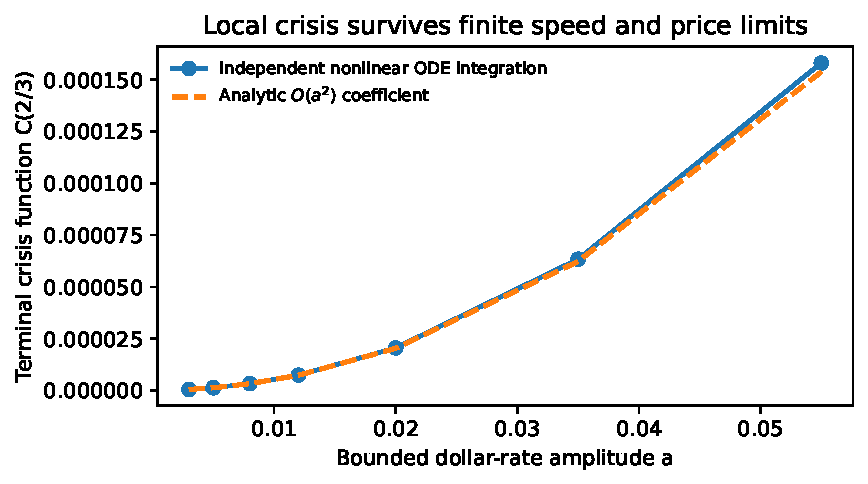
\includegraphics[width=0.76\linewidth]{../../paper/figures/finite_rate_quadratic.pdf}
\caption{\textbf{有限速度制御下の二次局所全資産損失。} 一定$g$の非線形価格経路を独立積分した結果は、\eqref{eq:finite-rate-coefficient}の解析的$a^2$係数へ収束する。表示振幅は価格正値性を保つほど小さい。強調した$a=0.035$の許容性検証はコード一式に記載する。}\label{fig:localrate}
\end{figure}


\FloatBarrier
\section{複数セッションの連続下限終値}\label{sec:multiday}
一セッションの価格下限は\emph{当日}の損失を制限するが、次のセッションは当日の低い終値から始まりうる。到達可能性分析を複数日へ延ばすには、\emph{どの}資産が下限へ繰り返し到達するか、危機汎関数が損失をどう集計するか、各売却の相手側に十分な売買代金受入容量があるかを追跡する必要がある。これらは連動する制約である。目標は対象資産数閾値を超え、各対象は十分速く売却され、補集合は自身の速度・値幅内でペアフローを受け入れなければならない。

ここで\emph{下限終値}とは、最後の約定価格がセッション下限と等しいことを指す。未約定売り注文列のある\emph{ストップ安張り付き注文板}ではない。約定取引状態には待ち行列ダイナミクスは含まれない。この区別はKim and Rhee~\citep{KimRhee1997}、Chen et al.~\citep{Chen2019}などの値幅制限の証拠を解釈する際に重要である。幾何学的ローリング値幅上限から条件付き危機判定へ、次いで速度・保存・資産間容量条件へ進み、最後に認証済み実行可能経路を示す。

\subsection{ローリング値幅と厳密な累積会計}\label{subsec:multiday-protocol}
取引時間を$D$個のセッション$[T_{d-1},T_d]$に分け、各長さを$\tau_d>0$とする。夜間の暦時間はモデル時計に加えず、価格は前の終値から連続的に引き継ぐ。仮想的な\emph{比例更新}版では$R_{i,d}=S_i(T_{d-1})$とし、次を要求する。
\begin{equation}\label{eq:rolling-band}
 (1-\beta_{i,d,-})R_{i,d}\le S_i(t)\le(1+\beta_{i,d,+})R_{i,d},
 \qquad t\in[T_{d-1},T_d],
\end{equation}
ここで$0<\beta_{i,d,-}<1$である。下限終値とは次式を指す。
$S_i(T_d)=(1-\beta_{i,d,-})R_{i,d}$。$D$日連続とは、\emph{同じ}資産について$D$連続セッションでこの等式が成り立つことをいう。$k=\lceil\alpha N\rceil$資産の連続下限終値だけでは定義\ref{def:crash}のシステミック危機ではなく、市場平均対数損失も所定閾値へ達する必要がある。

共通の一定下限比率$q=1-\beta_-$について、連続下限資産は次を満たす。
$S_i(T_D)=Fq^D$、損失$L_i(T_D)=D\lambda$、ただし$\lambda=-\log q$である。逆に連続下限でなくても、共通値幅と初期共通基準価格の下で状態制約は次を保証する。
\begin{equation}\label{eq:rolling-cumulative-upper}
  \Cris_\alpha(T_D)\le D\lambda
\end{equation}
値幅が異なる場合、右辺は次に置き換えられる。
$\max_i\sum_{d=1}^D[-\log(1-\beta_{i,d,-})]$。これらは\emph{幾何学的上限}であり、売買代金ペア決済経路が下限へ達する十分条件ではない。

実際の東京証券取引所規則では、日次円建て絶対値幅は共通割合ではなく基準値段の価格帯に依存し、基準値段は特別気配を反映する場合がある。基準が前日終値と等しい場合、下限終値の概念的再帰は$R_{i,d+1}=R_{i,d}-\Delta_-(R_{i,d})$である。約定がゼロまたは最少となる所定の連続二セッションを経て、特別手続により日次値幅が拡大されうる\citep{JPX2026}。比例更新モデルはこの条件付き市場規則を意図的に省略する。


\subsection{連続下限終値下の横断的危機閾値}\label{subsec:multiday-breadth}
第一の関門は\emph{定義}にある。$k$銘柄の連続下限終値は対象範囲条件を満たすが、平均損失条件を自動的には満たさない。残る資産はペア売買代金を受けて上昇しうる。これは市場Cの一部資産結果を可能にする$k<N$の補償機構を逆側から見たものである。以下の厳密な終端恒等式は、まだ取引を構成せずに、\emph{同じ}汎関数の下で下落多数派がいつ危機となるかを示す。
\begin{proposition}[条件付きシステミック危機発生判定]\label{prop:multiday-crisis-trigger}
同じ$k=\lceil\alpha N\rceil<N$資産の終値が$Fq^D$となるとする。これは$D$回の同一比例更新セッション後の価格で、$q\in(0,1)$とする。残る$N-k$資産の終値を$Y_j>0$とし、$\lambda=-\log q$と書く。任意の$0<\delta\le D\lambda$について、\emph{終端}危機閾値$\Cris_\alpha(T_D)\ge\delta$が成立する必要十分条件は次式である。
\begin{equation}\label{eq:multiday-trigger-product}
\boxed{\qquad \prod_{j=1}^{N-k}\frac{Y_j}{F}
 \le\exp\bigl(kD\lambda-N\delta\bigr).\qquad}
\end{equation}
他の全資産の個別対数損失が高々$D\lambda$である場合（または$k>N/2$で、他の$N-k$資産が上位$k$順位を埋められない場合）、$Q_\alpha(T_D)=D\lambda$であり、終端危機深度は厳密に次式となる。
\begin{equation}\label{eq:multiday-trigger-exact}
\boxed{\quad\Cris_\alpha(T_D)=\min\!\left\{D\lambda,
 \frac{kD\lambda-\sum_{j=1}^{N-k}\log(Y_j/F)}{N}\right\}.\quad}
\end{equation}
特に単一補償資産（$k=N-1$）の場合、その終端価格は$Y/F\le\exp(kD\lambda-N\delta)$を満たす必要がある。これは閾値$\delta$の危機が発生するための条件である。これらは厳密な\emph{条件付き終端恒等式}であり、所定終値を実現する取引経路の十分条件ではない。
\end{proposition}
\begin{proof}
連続下限の$k$資産の損失は$D\lambda$なので$Q_\alpha\ge D\lambda$である。$\delta\le D\lambda$では危機基準の対象範囲部分は自動的に満たされ、残る要件は$A\ge\delta$である。終端価格を$A=N^{-1}\sum_i\log(F/S_i)$へ代入すると\eqref{eq:multiday-trigger-product}を得る。他の全損失が高々$D\lambda$の場合、または$N-k<k$の場合、$k$番目に大きい損失は厳密に$D\lambda$となり、\eqref{eq:multiday-trigger-exact}を得る。
\end{proof}
命題\ref{prop:certified-v7}の区間認証付き$N=10$、$k=9$、$q=0.97$、$D=2$構成では、$D\lambda\approx0.060918$である。高精度再構成での補償資産終値は$Y/F\approx1.405161$で、$\Cris_{0.9}\approx0.020811$を与える。外向き丸め認証は$1.4047874<Y/F<1.4055543$を与え、指定経路で$\Cris_{0.9}>0.020$を厳密に含意する。閾値$\delta=0.020$には$Y/F\le\exp(9D\lambda-10(0.020))\approx1.416609$が必要で、認証経路はこれを満たす。したがって同じ広範な連続下限終値がシステミック損失となるかは、受入資産の終端価格で決まる。

\begin{figure}[tbp]\centering
 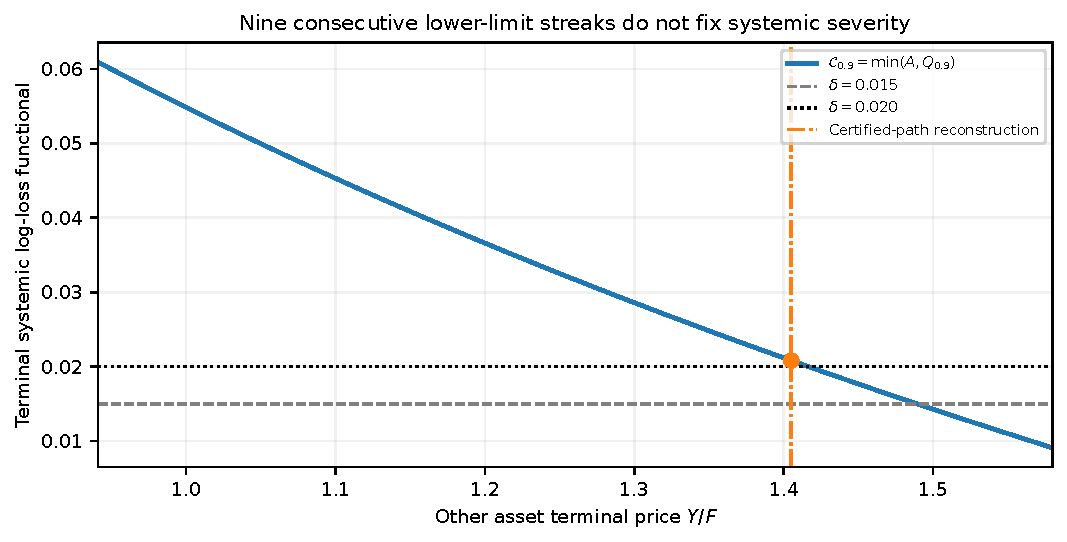
\includegraphics[width=0.85\linewidth]{../../paper/figures/multiday_crisis_trigger.pdf}
\caption{\textbf{連続下限終値だけではシステミック危機ではない。} $N=10$で、九資産が日次 3\%下限で二回引ける場合の条件付き終端深度を、残る資産の終端価格に対して示す。点線マーカーは構成した終端売買代金ゼロの実行可能経路である。 1.5\%と 2.0\%は対数損失閾値で、日次値幅ではない。曲線は代数的終端基準であり、全補償価格が動的に到達可能だとの主張ではない。}\label{fig:multiday-crisis-trigger}
\end{figure}

\subsection{連続下限終値の最小速度}\label{subsec:multiday-rate}
第二の関門は\emph{単一資産の執行容量}である。$F$への回復に抗して、有限時間内に下限終値へ達しなければならない。$g(S)\equiv\eta$で、セッション初値を$s$、長さを$\tau$、下限を$(1-\beta)s$とする。対応売買代金を誰が購入するかを問う以前に、総売買執行速度上限は$\dot z=-\rho(z-F)-\eta\bar v$、$z(0)=s$によって最速下落を制限する。これは必要閾値を与えるが、市場全体のマッチング問題は未解決のままである。
\begin{proposition}[ローリング下限のショック速度証明]\label{prop:rolling-rate}
株当たり一定インパクトモデルにおいて、初値$s>0$のセッションで下限終値となるには次が必要である。
\begin{equation}\label{eq:single-session-streak-rate}
 \boxed{\quad\bar v\ge \left[\frac{\rho}{\eta}\left(F-s+
 \frac{\beta s}{1-e^{-\rho\tau}}\right)\right]_+.\quad}
\end{equation}
同じ資産が$D$セッションのすべてで同じ比例下限で引け、共通セッション長が$\tau$で、$s_d=Fq^{d-1}$なら、次が成り立つ。
\begin{equation}\label{eq:D-streak-speed}
\boxed{\quad\bar v\ge\frac{\rho F}{\eta}\max_{1\le d\le D}
 \left[1+q^{d-1}\left(\frac{1-q}{1-e^{-\rho\tau}}-1\right)\right].\quad}
\end{equation}
さらに$\eta\bar v<\rho F$なら、$F$から始まる全価格は恒久的な\emph{速度のみの}下限$S_i(t)\ge F-\eta\bar v/\rho$に従う。これから連続日数の必要上界を得る。
\begin{equation}\label{eq:streak-D-bound}
\boxed{\quad D\le\frac{\log(1-\eta\bar v/(\rho F))}{\log q}.\quad}
\end{equation}
この上界は$\eta\bar v<\rho F$に限り意味を持ち、より大きい速度上限では有限日数の障壁を与えない。これらのスカラー不等式はいずれも、多資産値幅実行可能性や終端売買代金ゼロ条件の十分条件ではない。
\end{proposition}
\begin{proof}
定数変化法と$\dot\theta_i\ge-\bar v$から次を得る。
$S_i(\tau)\ge F+(s-F)e^{-\rho\tau}-(\eta\bar v/\rho)(1-e^{-\rho\tau})$.
$S_i(\tau)\le(1-\beta)s$を要求すると\eqref{eq:single-session-streak-rate}を得る。各日について$s=Fq^{d-1}$を代入すると\eqref{eq:D-streak-speed}となる。初期$F$からの同じスカラー比較は$S_i(t)\ge F-(\eta\bar v/\rho)(1-e^{-\rho t})$を与え、一様下限を得る。これを$Fq^D$と組み合わせ、$\log q<0$に注意すると\eqref{eq:streak-D-bound}を得る。
\end{proof}


\subsection{全資産連続下限が不可能となる理由}\label{subsec:multiday-full}
第三の関門は\emph{市場全体の保存則}である。全資産の場合は特に厳しく、純売買代金を受け入れる補集合がない。最初の安定性障壁を与えた同じポテンシャルが、基準以下の単純な値幅条件下で二回目の同時下落を排除する。別の経済機構ではなく、A/B/C領域で示した対象範囲の違いの大域的な端である。
\begin{theorem}[二回目の全資産下限終値への障壁]\label{thm:no-second-global}
$g_i(S)>0$、$\rho_i>0$、不変のファンダメンタル基準$F_i>0$、および瞬間的資産間売買代金均衡$\sum_i\dd X_i=0$を仮定する。全資産が第一セッションで$S_i(T_1)=q_iF_i<F_i$に引け、\emph{第二セッション許容値幅全体}が各基準以下にあるとする。
\begin{equation}\label{eq:no-second-condition}
 (1+\beta_{i,2,+})q_i\le1\quad\text{for every }i.
\end{equation}
すると\emph{全資産}が第二セッションで第一終値より厳密に低く引けることは不可能である。特に全$N$資産の同時第二日下限終値は不可能である。これは取引速度上限、終端符号付き売買代金残高、正の$g_i$の関数形に依存しない。
\end{theorem}
\begin{proof}
$\Phi_i'(S)=S/g_i(S)>0$および$H=\sum_i\Phi_i(S_i)$を用いる。取引決済は$H$を保存し、回復は次を与える。
$\dot H=-\sum_i\rho_i S_i(S_i-F_i)/g_i(S_i)\ge0$、ただしすべての$S_i\le F_i$の場合である。
条件\eqref{eq:no-second-condition}は第二セッションの価格経路全体をこの領域に保つ。ゆえに$H(T_2)\ge H(T_1)$である。すべての第二終値が前の終値未満なら、全$\Phi_i$の狭義単調性から逆に$H(T_2)<H(T_1)$となり、矛盾する。
\end{proof}

仮想的な対称比例値幅では、$q_i=1-\beta_i$および
$\beta_{i,2,+}=\beta_i>0$であるため、
$(1+\beta_i)(1-\beta_i)=1-\beta_i^2<1$であり、定理が適用される。この結論は、本研究の\emph{完全約定・資産間売買代金均衡・固定ファンダメンタルズ}市場の性質であり、現実の取引所で全株が再び同時下落できないとの予測ではない。未対応注文、外部取引脚としての現金、ファンダメンタルズは含まれない。また他資産が相殺売買代金を供給する間に$k<N$資産が連続下限となることは禁じない。


同じモデルは、全価格が厳密に$F_i$未満で固定された正の持続時間の\emph{全資産ストップ安張り付き状態}を表せない。$\dot S_i=0$を保つには次が必要となる。
各資産で$\dot X_i=\rho_i S_i(S_i-F_i)/g_i(S_i)<0$となり、$\sum_i\dot X_i=0$に矛盾する。一方、下限到達の終値約定は終端条件として許される。持続する未対応売り注文列には、価格軌道の延長だけでなく新たな注文板状態が必要である。

\subsection{正の複数日資源・会計制約}\label{subsec:multiday-preconditioning}
全資産が下落しなくても、$F$未満の各対象資産は上向き回復を受ける。したがって終端売買代金ゼロ条件には、最後の売却フローだけでなく経路履歴上の資源が必要となる。以前の基準超過が、後の損失を補償する正の回復寄与を供給しなければならない。これは第\ref{sec:barriers}節の同じポテンシャルを連続セッションにわたり積分した別の表現である。
\begin{proposition}[終端売買代金ゼロの連続下限に必要な事前準備]\label{prop:streak-precondition}
資産が$F$で始まり、$D$セッション後に$s_D<F$で終え、$X_i(T_D)=0$とする。この軌道は必ず正の取引時間測度を持つ集合上で$S_i>F$を訪れ、次を満たす。
\begin{equation}\label{eq:streak-excursion}
 \rho\int_0^{T_D}\frac{S_i(t)(S_i(t)-F)}{g(S_i(t))}\dd t
 =\int_{s_D}^{F}\frac{u}{g(u)}\dd u>0.
\end{equation}
第一セッション後の各セッションで資産が$F$以下に保たれ、第一セッション上限が$U_1>F$なら、必要条件は次式である。
\begin{equation}\label{eq:streak-precondition}
 \boxed{\quad \rho\tau_1\max_{F\le u\le U_1}\frac{u(u-F)}{g(u)}
 \ge \int_{s_D}^{F}\frac{u}{g(u)}\dd u.\quad}
\end{equation}
一定インパクト$g=\eta$、$s_D=Fq^D$、$U_1=F(1+\beta_+)$では次へ簡約される。
$\rho\tau_1\ge(1-q^{2D})/[2\beta_+(1+\beta_+)]$。
$H_+=\rho\tau_1\beta_+(1+\beta_+)$と書くと、$2H_+<1$の場合に次の追加的な必要連続日数上界が課される。
\begin{equation}\label{eq:multiday-preconditioning-D}
\boxed{\quad D\le \frac{\log(1-2H_+)}{2\log q}.\quad}
\end{equation}
この上界は終端売買代金ゼロ条件と、後のセッションでファンダメンタル基準を超えないことに固有である。連続下限経路を作る十分条件ではない。
\end{proposition}
\begin{proof}
恒等式$\dd\Phi(S_i)=\dd X_i-\rho S_i(S_i-F)\dd t/g(S_i)$を全期間で積分する。$X_i(T_D)=0$かつ$\Phi(F)=0$なので、積分は$-\Phi(s_D)>0$と等しい。$S_i\le F$の経路部分は非正の被積分関数を与えるため、正部分は$F$より上で生じなければならない。後のセッションが$F$を超えられないなら、正寄与はすべてセッション 1 で得る必要があり、その上限は\eqref{eq:streak-precondition}の左辺で制限される。
\end{proof}


\subsection{多資産執行に必要な受入容量の下界}\label{subsec:multiday-cut}
先の検査は下落株を個別に、または市場全体を集団として制約する。しかしシステミック危機の中核となる中間の場合、すなわち\emph{大半}が下落し少数の補集合が反対側の売買代金を決済する場合を捉えない。これはA/B/C構成の$k<N$の場合そのものである。構造的到達可能性は補償資産の存在を許すが、執行可能性は、その許容総売買執行速度と値幅がどれほど吸収できるかを問う。資産を下落部分集合$J$と補集合$J^c$に分ける。保存則と資産別総執行速度は、分割を横切る売買代金を直接制限する。これは、節点別総速度上限を持ち、独立な辺容量を持たない完全取引グラフの\emph{必要部分集合容量不等式}である。構造的に許される一部資産損失を、非下落資産の必要売買代金受入能力へ結びつける。
\begin{proposition}[市場カット容量と連続下限の下界]\label{prop:market-cut}
資産部分集合$J$を固定し、補集合を$J^c$と書く。売買代金ペア決済と資産別総売買執行速度上限$\bar v$の下、任意の許容絶対連続経路は、ほとんどすべての$t$で次を満たす。
\begin{equation}\label{eq:market-cut-instant}
\boxed{\left|\sum_{i\in J}\dot X_i(t)\right|\le
\bar v\min\left\{\sum_{i\in J} S_i(t),\sum_{j\in J^c}S_j(t)\right\}.}
\end{equation}
セッション$[T_{d-1},T_d]$は長さ$\tau_d$を持ち、その全体で各資産$i\in J$の価格が不変基準$F_i$以下にあり、$s_{i,d}<s_{i,d-1}$で終えるとする。$\Phi_i'(S)=S/g_i(S)>0$とし、次を置く。
\begin{equation}\label{eq:cut-required}
K_{J,d}:=\sum_{i\in J}\big[\Phi_i(s_{i,d-1})-\Phi_i(s_{i,d})\big]>0.
\end{equation}
このセッション中、全補償資産が$S_j(t)\le U_{j,d}$を満たすなら、セッションのペア売買代金$M_d$と必要総売買執行速度上限は次を満たす。
\begin{equation}\label{eq:cut-necessary}
\boxed{M_d\ge K_{J,d},\qquad
\bar v\ge\frac{K_{J,d}}{\tau_d\sum_{j\in J^c}U_{j,d}}.}
\end{equation}
$J^c=\varnothing$の場合、仮定した全資産の同時厳密下落は、全体が基準以下のセッションでは生じえない。
\end{proposition}
\begin{proof}
売買代金ペア化から$\sum_{i\in J}\dot X_i=-\sum_{j\in J^c}\dot X_j$である。いずれの集合でも$|\dot X_i|\le S_i r_i^{\mathrm{gross}}\le S_i\bar v$であり、\eqref{eq:market-cut-instant}を得る。価格応答座標は次を満たす。
$\Delta X_i=\Phi_i(s_{i,d})-\Phi_i(s_{i,d-1})+
\rho_i\int_{T_{d-1}}^{T_d}S_i(S_i-F_i)/g_i(S_i)\dd t$.
積分は$i\in J$で非正なので、$\sum_{i\in J}\Delta X_i\le-K_{J,d}$となる。したがって$J^c$へ入る純売買代金は少なくとも$K_{J,d}$である。総ペア売買代金はこのフローを賄う必要があり、補集合の総株数執行による売買代金受入容量は高々$\bar v\tau_d\sum_{j\in J^c}U_{j,d}$である。これらから\eqref{eq:cut-necessary}を得る。$J^c$が空なら反対フローは存在しない。
\end{proof}
ここで構造と執行の議論が結びつく。$J^c$が空ならカットに受入側はなく、全資産障壁に対応する。$J^c$が空でなければ、構造的に許される経路でも補集合の利用可能容量を超える速度を必要としうる。同じ残存資産は危機汎関数に逆向きの第二効果を持つ。その価格上昇は命題\ref{prop:multiday-crisis-trigger}で測る下落多数派の平均対数損失を相殺しうる。したがって実行可能性には、十分な資金吸収と十分に相殺されない平均損失の\emph{両方}が必要である。

株当たり一定インパクト$g_i\equiv\eta$、同一の下限対象資産数$k=|J|$、初期基準$F$、共通下限比率$q\in(0,1)$、および$m=N-k$個の補償資産で共通上限割合$\beta_{c,+}$を持つ場合、第$d$日の特殊形は次式となる。
\begin{equation}\label{eq:cut-special}
\boxed{\bar v\ge \frac{k}{m}\,
\frac{F\,\big(q^{2(d-1)}-q^{2d}\big)}{2\eta\tau_d(1+\beta_{c,+})^{d}}\quad(d\ge2),}
\end{equation}
ただし全$k$対象価格は$F$未満を保ち、各補償資産の前日基準価格が所定上限値幅の下で$F$から発展しているものとする。$k/m$倍の係数は資金受入のボトルネックを明示する。これは\emph{必要}条件であり、厳密最適値ではない。十資産二日間の例（$k=9,m=1,q=0.97,\beta_{c,+}=0.25,\tau_d=20$）では$\bar v\gtrsim 0.0080$にとどまる。この設定では後述のより強いシステミック二次上界の方が有益である。

\subsection{検証済み低速度構成と最小速度の両側区間}\label{subsec:v7-certified}
必要制約は同時実行可能性を証明しない。そこで、それらをすべて守る\emph{単一経路}を認証する。$N=10$とし、九つの同一対象資産と一つの補償資産、$F=\eta=1$、$\rho=0.4$、長さ$20$の二セッション、対象資産のローリング値幅$\pm3\%$、補償資産値幅$\pm25\%$、および各資産の終端条件$X_i(40)=0$を固定する。対象資産は所定の連続価格経路$x(t)$を共有し、補償資産はペア売買代金で定まるスカラー非線形ODEに従う。構成は二価格状態へ縮約されるが、十資産モデル全体の非空な許容集合を認証するものであり、不均質パラメータへの一般的頑健性を認証するものではない。以下の区分線形対象経路について、非線形補償ダイナミクスと執行制約を独立再実行可能な固定小数点区間計算で認証できる。
\begin{proposition}[計算機支援による二日間速度認証]\label{prop:certified-v7}
第\ref{subsec:v7-certified}節で指定した十資産設定（$k=9$、$F=\eta=1$、$\rho=0.4$、$\tau_1=\tau_2=20$、対象値幅$\pm3\%$、補償値幅$\pm25\%$）において、すべての資産の終端符号付き売買代金元帳が厳密にゼロとなる連続・絶対連続・完全ペア決済経路が存在する。同じ九資産が第一セッションでは$0.97$、第二セッションでは$0.9409$で引け、次を満たす。
\begin{equation}\label{eq:v7-certified-result}
\boxed{\Cris_{0.9}(40)>0.020,\quad \bar v_{\mathrm{used}}<0.285,\quad M<3,\quad H_i^-<2\quad(1\le i\le10).}
\end{equation}
全約定価格は各ローリングセッション値幅内にある。$M$はペア売買代金を一回数え、$H_i^-$は総売却株数を表す。したがって各資産二株の初期保有で空売りを避けられる。
\end{proposition}
\begin{proof}[証明の概要；再現可能な検証包含は付録~\ref{app:v7certificate}]
$r=23/10$とする。共通対象価格$x(t)$を次の点の連続区分線形補間で指定する。
\begin{equation}\label{eq:v7-knots}
(t,x)=(0,1),(r,h),(20-r,h),(20,0.97),(20+r,0.995),(40-r,0.995),(40,0.9409).
\end{equation}
第一平坦価格$h$は、次の厳密な純売買代金ゼロ方程式の$1.02$付近の一意な根である。
\begin{equation}\label{eq:v7-root}
101600000000h^2-97138000000h-6646157699=0,
\quad1.02020225507905<h<1.02020225507908.
\end{equation}
補償価格$y(t)$は次の一意な正の解である。
$\dot y=-0.4(y-1)-9u(t)/y$、$y(0)=1$、ただし
$u(t)=x(t)[\dot x(t)+0.4(x(t)-1)]$である。
全十資産の売買代金フローは各時点で和がゼロであり、厳密な根方程式は全対象資産について$X_i(40)=0$を与える。ゆえに補償資産もゼロとなる。検証済み区間積分から次を得る。
\begin{equation}\label{eq:v7-bounds}
\begin{gathered}
1.2219388<y(20)<1.2225356,\quad
1.4047874<y(40)<1.4055543,\\
\sup_t9|u(t)|/y(t)<0.284481,\\
\int_0^{40}9[u(t)]_+/y(t)\dd t<1.880,\qquad
9\int_0^{40}|u(t)|\dd t<2.984.
\end{gathered}
\end{equation}
対象資産の総執行速度と総売却株数はさらに小さい。セッション別区間包含により両ローリング値幅を検証する。$e^{0.2}$の厳密な有理包含は$\overline L(40)>0.020$を検証し、九対象資産の損失は$-\log(0.9409)>0.020$であるため、\eqref{eq:v7-certified-result}が示される。
\end{proof}
この\emph{固定した}十資産・二日・九連続下限資産の例で、$\bar v_*$を、$\Cris_{0.9}(40)\ge0.020$も満たす\emph{全}許容経路にわたる総執行速度上限の下限とする。市場全体の二次上界\eqref{eq:quadratic-rate}は、すべての$\bar v\le 0.044$について（$F=\eta=1$、$\rho=0.4$、$T=40$で）次を含意する。
\[
\Cris_{0.9}(40)\le (\bar v/0.4)^2
\left[1+\frac{1}{2(1-\bar v/0.4)^2}\right]
\le \frac{1563441}{79210000}<0.020.
\]
\eqref{eq:quadratic-rate}の右辺は、$\bar v$について$0.044$近傍で連続であり、この値で$0.020$を厳密に下回るため、排除は$0.044$を上回る一部の速度にも及ぶ。命題\ref{prop:certified-v7}の実行可能構成と合わせると、最小総執行速度上限について次の厳密だが非最適な挟み撃ちを得る。

\begin{equation}\label{eq:v7-rate-bracket}
\boxed{\qquad 0.044<\bar v_*<0.285.\qquad}
\end{equation}
この区間は固定市場での問いの連鎖を完結する。応答則は一部資産暴落を許す。危機定義は十分な平均損失を要求する。日次値幅と総執行速度は許容経路を制約する。ペア決済は受入側を制約する。そして認証経路が実際に目標へ達する。下界と上側構成例は異なる論理的役割を持つ。認証制御は実行可能な速度上界を、二次障壁は厳密な下界を与える。厳密な大域的最小値の決定は制約付き複数日最適制御問題として残る。
\paragraph{感度と対称性の役割。}
十資産認証は九つの同一対象状態を意図的に一軌道へ縮約する。\emph{同じ}$x(t)$と厳密な対象売買代金ゼロ条件を固定し、数値感度検査では十資産を$k$個の同一対象と$10-k$個の同一補償資産へ再分割する。共通補償価格は$\dot y=-0.4(y-1)-[k/(10-k)]u(t)/y$に従う。表\ref{tab:sensitivity}は受入資産数の重要性を示す。検査例の中で、指定制御が固定の$0.020$平均損失目標を達成するのは$k=9$だけである。$k$の変更は対象比率$k/10$も変えるため、$\alpha=0.9$を固定した検査ではない。これは、再設計した経路でも$k<9$で不可能だとの証明\emph{ではない}。これらの行は高精度ODE診断であり、$k=9$の区間認証とは異なる。同様に固定$k=9$経路について、認証は対称補償値幅$\pm24.7\%$で適合を、$\pm24\%$で違反を証明する（$t=17.7$の価格区間が$0.76$を厳密に下回る）。値幅変更は制御の再実行や最適化を伴わない。
\begin{table}[H]\centering\small
\caption{\emph{固定した認証対象制御形状}の横断構成への感度。$k=9$行だけが区間認証済みで、他は独立積分した高精度スカラーODEを用いる。共通補償値幅は\emph{計算された}経路と両立する最小対称日次割合である。値は診断であり、最適実行可能閾値ではない。}\label{tab:sensitivity}
\begin{tabular}{@{}rrrrr@{}}\toprule
対象数$k$ & 補償資産数 & $y(40)$ & 平均対数損失 & 計算上必要な値幅 \\\midrule
 6  &  4  &  1.08112  &  0.00535  &  4.28\%\\
 7  &  3  &  1.12302  &  0.00784  &  6.55\%\\
 8  &  2  &  1.20141  &  0.01204  &  10.88\%\\
 9  &  1  &  1.40516  &  0.02081  &  24.55\%\\
\bottomrule\end{tabular}
\end{table}

\begin{figure}[H]\centering
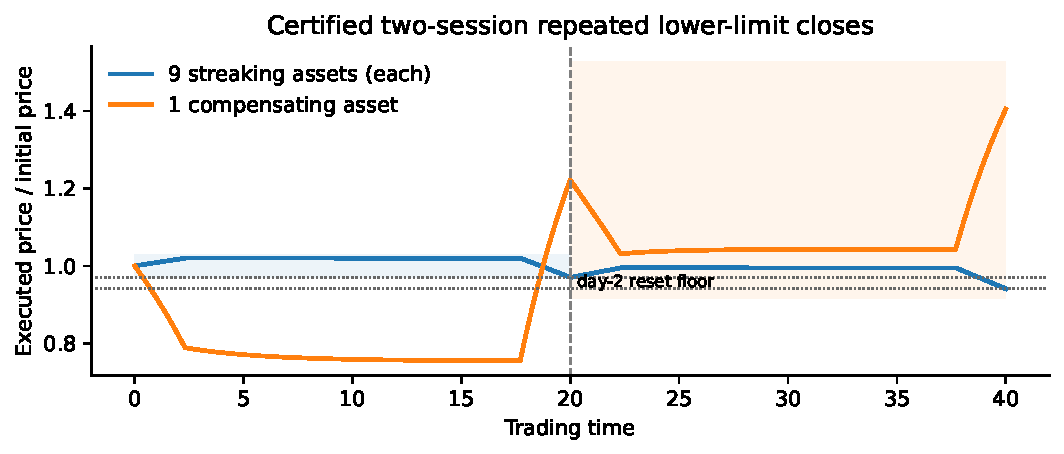
\includegraphics[width=0.87\linewidth]{../../paper/figures/v7_certified_multiday_prices.pdf}
\caption{\textbf{区間認証された低速度経路。} 改良二日間構成の連続対象価格と補償価格。九対象資産は更新下限で引け、補償資産は 25\%の日次制限内にとどまる。曲線は例示的な数値再構成であり、許容性は付録\ref{app:v7certificate}の外向き丸め計算で独立に認証される。}\label{fig:v7path}
\end{figure}
\begin{figure}[H]\centering
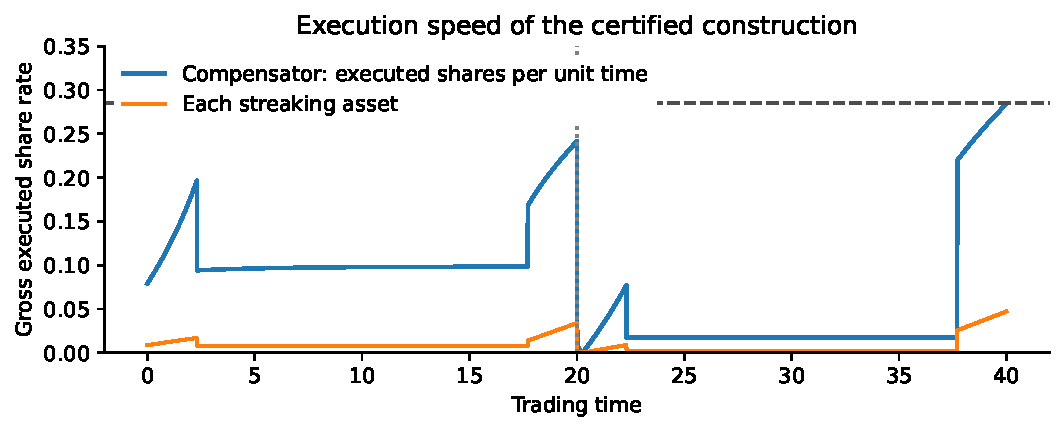
\includegraphics[width=0.87\linewidth]{../../paper/figures/v7_certified_rate_path.pdf}
\caption{\textbf{認証経路の総執行速度。} 計算上の最大総売買執行速度は約$0.28422$である。厳密区間丸めにより、瞬間パルスなしで$0.285$未満の上界を認証する。上限は資産別で、購入・売却の相殺前に課す。}\label{fig:v7rates}
\end{figure}
\clearpage

\section{解釈、限界、検証可能な含意}\label{sec:discussion}
一般化座標標準形\eqref{eq:normal-form}は結果を一つの系列に整理する。売買代金は加法的に入り、応答適合型座標の和を保存し、回復が取引間でその和を駆動する。曲率は大域的安定性障壁を与え、A/B/C族は応答幾何による障壁の変化を示し、座標距離はシステミック損失集合への到達に必要な執行資源を制限する。有限速度と日次更新値幅は許容経路をさらに制約する。認証済み二日構成はこれらを同時に満たせることを示し、部分集合容量不等式は下落多数派と残存資産の購買容量を結びつける。

均衡に由来する機構との違いは明確である。Huang and Wang~\citep{HuangWang2009}は非同期需要、Cespa and Foucault~\citep{CespaFoucault2014}は資産間学習、Cont and Wagalath~\citep{ContWagalath2013}は窮迫売却が誘発する相関、Cordoni and Lillo~\citep{CordoniLillo2024}はインパクトゲームの戦略的不安定性を研究する。本研究はそれらの選択機構を捨象し、指定した\emph{制御市場}で危機状態を排除する条件、またはそこへの制約付き経路を許す条件を特定する。Kyle and Obizhaeva~\citep{KyleObizhaeva2023}は不変性と観測暴落により大口取引・執行速度の価格含意を定量化するが、本研究の容量・低速度下界は観測暴落への較正済み定量予測を与えない。貢献は、共通決済・回復規則の下で構造・資源・執行を合わせた到達可能性を問うことであり、既存機構の代替ではない。

十資産構成例は対称な九対象軌道と一補償資産を用い、計算を二価格状態へ縮約する。表\ref{tab:sensitivity}の感度検査は固定対象制御下の補償負担の変化を定量化する。認証イベントは\emph{システミック・ドローダウン}である。九銘柄が二セッションでそれぞれ$5.91\%$を失う一方、第十銘柄は上昇し、等ウェイト幾何平均は約$2.06\%$下落する。

実証応用には、高頻度データから$g(S)$、回復$\rho$、実行可能な資産間注文フロー、在庫、現金決済を同定する必要がある。静的注文板スナップショットや日次OHLCV系列ではこれらの入力の同定に不十分であり、有効応答$g$は自動的にKyleのlambdaではない。構成の値幅は\emph{約定価格}に課す仮想割合制限だが、実際の東京証券取引所制限は通常、価格帯別の円建て絶対範囲と所定拡大規則を用いる\citep{JPX2026}。モデル化した下限終値は未約定売り列や実際の張り付き市場を意味しない。

個別の株数中立往復取引の執行費用が非負でも、売買代金中立再配分は最終保有株数を変え、取引資産価値を散逸させうる。本結果は制御市場の許容価格状態を特徴づける。行動上の選択と実証イベント頻度には追加モデルが必要である。

\paragraph{対角インパクトとポテンシャルに基づく拡張。}
本研究の資産間依存は売買代金ペア化から生じ、限界インパクト行列は対角である。直接クロスインパクト$\dd\bm S=\mathsf G(\bm S)\dd\bm\theta$と可逆な$\mathsf G$を持つモデルでは、取引会計は微分一形式$\omega=\one^\top\operatorname{diag}(\bm S)\mathsf G(\bm S)^{-1}\dd\bm S$を示唆する。スカラー取引ポテンシャルには、この微分一形式が完全微分となるための適切な条件と、回復ドリフトに整合的な符号条件が必要である。行列インパクト係数の対称性や正定値性だけではこれらは保証されない。この点は、本研究の分離可能ポテンシャルの結果を、Alfonsi, Kl\"ock, and Schied~\citep{AlfonsiKlockSchied2016}の行列核条件やCordoni and Lillo~\citep{CordoniLillo2024}のクロスインパクトNashゲームと区別する。

\section{結論}\label{sec:conclusion}
応答適合型一般化価格座標は非線形取引インパクトを、加法的で売買代金均衡する移転と復元ドリフトへ還元する。曲率は大域的排除障壁を特定し、座標距離は必要資源下界を与える。共通応答族は三つの到達可能性領域を示し、速度制約付き複数日区間認証構成は、より厳しい執行制約下でもシステミック・ドローダウンが存続しうることを示す。構造的実行可能性、利用可能資源、複数日執行容量は、市場安定性に対する連続した数学的に異なる検査を構成する。

\section*{コードと数値データの利用可能性}
同梱の再現性パッケージは、\path{verification/certify_streak_interval.py}（厳密有理根分離と外向き丸め固定小数点包含）、\path{verification/verify_consistency.py}、数値感度スクリプト、作図コード、機械可読出力、LaTeXソース、およびファイルハッシュ一覧を含む。再現コマンドとソフトウェア要件は\path{REPRODUCE.md}にある。認証はソースから再実行され、独立した浮動小数点ODE検査と厳密有理整合性検査も行われた。版とチェックサムで索引付けされた再現性アーカイブを原稿に添付する。計算は供給ソース・認証の版に結びついている。

\section*{AI支援ツールに関する声明}
AI支援ツールを、原稿の一部の起草・構成、数学計算の開発・検証、計算スクリプトの作成、および図の準備に用いた。著者は数学的主張、出典の帰属、および数値認証の再現性を含む、すべての内容に責任を負う。

\appendix
\section{決済、座標変換、変動の下界}\label{app:accounting}
連続応答則は有限変動執行経路に沿って解釈する。理想化パルスの間、物理時間は凍結され（$\dd t=0$）、状態は執行株数の変化に応じて応答ODEに沿って動く。パルスの売買代金移転は\emph{積分}$\int S_i\dd\theta_i$であり、開始価格と最終株数増分の積ではない。$g>0$の連続性により、中間価格が正を保つなら、その端点は許容応答経路で結べる。

単一資産の微分則は次式となる。
\begin{equation}\label{eq:appendix-s}
\dd\theta=\frac{\dd S+\rho(S-F)\dd t}{g(S)}.
\end{equation}
$S=F+(S-F)$と分解して積分する。
\begin{align*}
\int_0^T S\dd\theta
&=F[\theta(T)-\theta(0)]
+\int_F^{S(T)}\frac{u-F}{g(u)}\dd u
+\rho\int_0^T\frac{(S-F)^2}{g(S)}\dd t,
\end{align*}
ここで初期価格は$F$である。これが\eqref{eq:cost}を証明する。$S<F$では、\eqref{eq:E}の原始関数$E(S)$も非負である。積分方向の反転が負の被積分関数の符号を反転するためである。したがって$\theta(T)=\theta(0)$なら総執行費用は負にならない。

$y=\Phi(S)$、$z=\Psi(S)$とし、次を用いる。
\[
\Phi'(S)=\frac{S}{g(S)},\qquad \Psi'(S)=\frac1{g(S)}.
\]
すると次が成り立つ。
\begin{equation}\label{eq:appendix-yz}
\dd y=\dd X-\rho\frac{S(S-F)}{g(S)}\dd t,
\qquad
\dd z=\dd\theta-\rho\frac{S-F}{g(S)}\dd t.
\end{equation}
回復項の符号は$S-F$と逆である。したがって$y<0$（同値に$S<F$）のとき、$y$の非取引ドリフトは正であり、$z$も同様である。\eqref{eq:appendix-yz}の正負変動を分けると、$y(T)\le\Phi(s)<0$で終える軌道は負の売買代金変動を少なくとも$-\Phi(s)$蓄積する必要がある。これは、$y$がゼロとなる\emph{最後の}時刻（その後ゼロにならなければ$t=0$）から始めると分かる。残りの区間で$y\le0$となり、回復ドリフトは非負である。ゆえに負の取引変動が$y(T)$までの全下落を担う必要がある。$z$でも同じ議論から株数売却下界を得る。条件を満たす資産の売却を合計すると、ペア売買代金移転をちょうど一回数える。終端条件を満たす資産の在庫上限が$H_i$で$X_i(T)=0$なら、式\eqref{eq:cost}から次を得る。
\[
E(S_i(T))\le F\left[\theta_i(0)-\theta_i(T)\right]\le FH_i.
\]
$E(S)$は、価格$S$が$F$未満へ下がるにつれて増加する。したがって$S_i(T)\le s$は$E(s)\le FH_i$を含意する。これにより定理\ref{thm:resource}が示される。

$\rho=0$なら$\dd\Phi(S_i)=\dd X_i$である。終端売買代金ゼロ条件から$\Phi(S_i(T))=\Phi(F)=0$となり、狭義単調性により$S_i(T)=F$となる。現在の分離可能応答クラスでは、回復が非自明な売買代金ゼロ終端効果を可能にする。

\section{局所二パルス・三パルス展開}\label{app:local}
命題\ref{prop:two-pulse}と\ref{prop:three-pulse}で用いた展開を記す。局所変動を$x=S/F-1$、$c=g(F)/F^2$で規格化する。$S=F$では、売買代金座標$y=\Phi(S)$は$\Phi(F)=0$、$\Phi'(F)=F/g(F)$、および次を満たす。
\begin{equation}\label{eq:local-inverse}
\frac{\dd S}{\dd y}=\frac{g(S)}S,
\qquad
\frac{\dd^2 S}{\dd y^2}=
\frac{g(S)[Sg'(S)-g(S)]}{S^3}.
\end{equation}
したがって$e_0=e(F)$と書くと、小さい売買代金座標変位$y$後の価格比は次式である。
\begin{equation}\label{eq:local-Taylor}
\frac SF=1+cy+\frac12(e_0-1)c^2y^2+O(y^3),
\end{equation}
定数は$F$のコンパクト近傍内の経路に対して一様有界である。

二パルス実験では、最初のインパルスが時刻ゼロに$y$を$hu_i$だけ変位させる。これは\eqref{eq:local-Taylor}による初期価格応答を生む。期間$T$の回復は\emph{水準}変位$S-F$を$r=e^{-\rho T}$倍し、終端パルスは同じ売買代金$hu_i$を売買代金座標から差し引く。$\Phi$と$\Phi^{-1}$を$F$近傍で展開すると次を得る。
\begin{align}\label{eq:local-two}
L_i(T)&=c(1-r)hu_i+\frac{c^2h^2}{2}\,\lambda(r,e_0)u_i^2+O(h^3),\\
\frac1N\sum_i L_i(T)&=\frac{c^2h^2}{2N}(1-r)(2-e_0-r)\sum_i u_i^2+O(h^3),\nonumber
\end{align}
ここで個別二次係数$\lambda$を単独で求める必要はない。$\sum_i u_i=0$なので平均で線形項は消える。少なくとも$k$成分が正なら、その資産には正の一次損失があり、第$k$大の損失は、小さい$h$で正となる。所定の時間・曲率条件下で平均も正である。

三パルス実験では、$0,T/2,T$の売買代金座標インパルスの量は$hu_i$、$-(1+r)hu_i$、$rhu_i$であり、$r=e^{-\rho T/2}$とする。直接代入と二次展開により次を得る。
\begin{equation}\label{eq:local-three}
L_i(T)=\frac{1-e_0}{2}c^2h^2u_i^2r(1-r^2)+O(h^3),
\end{equation}
一次項は厳密に相殺する。$e_0<1$で、すべての$u_i\ne0$なら、十分小さい$h$で全終端損失は正である。各パルス量ベクトルはゼロ和で、全期間にわたる量は成分ごとに相殺するため、構成は売買代金ペア決済と終端ゼロ条件も満たす。固定$h$で初期在庫要件と売買代金は有限である。

\section{一様資源下の一部資産の深刻ドローダウン}\label{app:severe}
定理\ref{thm:ABC}(C)を構成的に証明する。$N\ge2$を固定し、$m=N-1$とし、一定応答モデル$g(S)=\eta>0$を選ぶ。大きい閾値を超える経路はすべての小さい閾値も超えるので、目標危機閾値$\delta$は大きいと仮定してよい。最終「補償」資産とともに、$m$個の終端価格$\varepsilon\downarrow0$を実現すれば十分である。すべての$k<N$が$k\le m$を満たすためである。

\subsection{ペア売買代金取引の半径表現}
$g\equiv\eta$について、次が成り立つ。
\begin{equation}\label{eq:radius-appendix}
\dd(S_i^2)= -2\rho S_i(S_i-F)\dd t+2\eta\dd X_i,
\qquad \one^\top\dd\bm X=0.
\end{equation}
$R=(\sum_iS_i^2)^{1/2}$とする。ペア売買代金取引は$R$を一定に保つ。固定$R$での正価格変化は、その球面の正象限内の有限変動経路として実装できる。特に同じ和の二つの正ベクトル間で二乗価格$Y_i=S_i^2$を線形補間する。中間点はすべて$Y_i>0$で$\sum_i\dd Y_i=0$なので、$\dd X_i=\dd Y_i/(2\eta)$は許容ペア移転である。対応する株数増分は$\dd\theta_i=\dd S_i/\eta$である。

小さい定数$c>0$とパラメータ$b\in(0,\beta)$を選ぶ。$\beta=1/5$としてよく、次を満たすようにする。
\begin{equation}\label{eq:abcs}
a=\sqrt{1-b^2-(m-1)c^2}>b>c>0,
\quad
H=a+(m-1)c+b,
\quad bH<1.
\end{equation}
十分小さい$c$でそのような選択は存在する。段階$j\in\{1,\dots,m\}$で球面方向を次のように固定する。
\begin{equation}\label{eq:uj}
\bm u_j=(c,\ldots,\underbrace{a}_{j},\ldots,c,b),
\qquad \|\bm u_j\|_2=1.
\end{equation}
段階全体で$\bm S(t)=R(t)\bm u_j$とする。これが価格方程式を解くよう、次を用いる。
\begin{equation}\label{eq:R}
R(t)=F\left[H+(\sqrt N-H)e^{-\rho t}\right],
\qquad
\dot\theta_i=\frac{\rho F}{\eta}\left(u_{j,i}H-1\right).
\end{equation}
実際、価格方程式で$S_i=u_{j,i}R(t)$を微分すると\eqref{eq:R}と次を得る。
\begin{equation}\label{eq:dXdt}
\dot X_i=\frac{\rho FR(t)}\eta\,u_{j,i}(u_{j,i}H-1),
\quad \sum_i\dot X_i=\frac{\rho FR(t)}\eta\left(H\sum_i u_{j,i}^2-\sum_i u_{j,i}\right)=0,
\end{equation}
これは$\sum_i u_{j,i}^2=1$かつ$\sum_i u_{j,i}=H$による。

\subsection{補償資産の売買代金フローのゼロ化}
$t=0$で$F\one$から始め、固定半径$F\sqrt N$の正価格パルスで第一方向$\bm u_1$へ移す。段階$\bm u_j$間の切替にも同様の固定半径パルスを用いる。時刻$T$で最後の固定半径パルスにより次へ達する。
\begin{equation}\label{eq:endpoint-severe}
S_1(T)=\cdots=S_m(T)=\varepsilon,
\quad S_N(T)=\sqrt{R(T)^2-m\varepsilon^2}.
\end{equation}
十分小さいすべての$\varepsilon$について終端価格ベクトルは正である。

一定$g$では、\eqref{eq:radius-appendix}の積分により厳密な売買代金元帳を得る。
\begin{equation}\label{eq:Xledger}
X_i(T)=\frac{S_i(T)^2-F^2}{2\eta}
+\frac\rho\eta\int_0^T S_i(t)[S_i(t)-F]\dd t.
\end{equation}
補償資産の段階重みは常に$b$である。次を定義する。
\begin{align}\label{eq:compensator}
\mathcal F_\varepsilon(b)=\frac{R_b(T)^2-m\varepsilon^2-F^2}{2\eta}
+\frac\rho\eta\int_0^T bR_b(t)[bR_b(t)-F]\dd t,
\end{align}
ここで$R_b$は$b$に、\eqref{eq:R}を通じて連続依存する。十分小さい$c$と$\varepsilon$について$\mathcal F_\varepsilon(0)>0$であり、その理由は$R_0(T)>F$である。$b=\beta$では\eqref{eq:abcs}から$bH<1$となり、終端項は有界のまま、時間積分は$T$に比例する速度で負になる。したがってある固定した十分長い$T$で、$\mathcal F_\varepsilon(\beta)<0$が小さい全$\varepsilon$に一様に成り立つ。連続性から、$b(\varepsilon)\in(0,\beta)$で$X_N(T)=0$を厳密に満たすものが存在する。

\subsection{全対象資産の売買代金フローのゼロ化}
残る$m$個の終端売買代金残高を等しくすればよい。資産が高状態$a$にある場合と低状態$c$にある場合の回復被積分関数の差は次式である。
\begin{equation}\label{eq:W}
W(t)=(a-c)R(t)\big[(a+c)R(t)-F\big].
\end{equation}
これは厳密に正である。$(a+c)H=1+b(a-b)+mac+bc>1$かつ$R(t)\ge FH$なので、$W(t)>0$が$t\in[0,T]$の全域で成り立つ。次を満たす分割$0=t_0<\dots<t_m=T$を選ぶ。
\begin{equation}\label{eq:weights}
\int_{t_{j-1}}^{t_j}W(t)\dd t=\frac1m\int_0^T W(t)\dd t,
\qquad j=1,\ldots,m.
\end{equation}
連続で狭義単調増加な累積積分により、この分割が可能である。対象資産$j$は段階$j$で高状態、その他で低状態を占めるとする。全対象資産は同じ初期価格$F$、終端価格$\varepsilon$、および\eqref{eq:Xledger}の回復積分を持つため、終端残高$X_i(T)$は等しい。各パルスと段階は$\sum_i\dd X_i=0$を守り、$X_N(T)=0$なので、共通対象残高もゼロでなければならない。したがって次を得る。
\begin{equation}\label{eq:allclosed}
X_i(T)=0\qquad\text{for every } i=1,\ldots,N.
\end{equation}

\subsection{一様有限売買代金と在庫}
経路は半径が高々$F\sqrt N$の正球面上にあり、全期間で$0<S_i\le F\sqrt N$である。固定半径パルスは$m+1=N$回で、各パルスは二乗価格座標の成分別単調補間で実装できる。したがって累積ペア売買代金パルスには、$N,F,\eta$だけに依存する明示的だが緩い上界がある。例えば安全な上界は$N^3F^2/(4\eta)$である。回復制御段階では$\sum_i|\dot X_i|/2\le \rho NF^2/\eta$なので、次を得る。
\begin{equation}\label{eq:uniformM}
M(\gamma)\le M_0:=\frac{N^3F^2}{4\eta}+\frac{\rho NF^2T}{\eta}.
\end{equation}
同様に、$N$回のパルスと連続段階の株数売却は次で制限される。
\begin{equation}\label{eq:uniformH}
H_i^-\le H_0:=\frac{NF\sqrt N+\rho FT(\sqrt N+1)}\eta,
\end{equation}
これは$\varepsilon$に依存しない。各資産を少なくとも$H_0$株から開始すれば空売りを排除できる。補償価格は有界で正を保ち、その対数損失は有限である。他の$m$損失は$\log(F/\varepsilon)\to\infty$となる。ゆえに$k$番目の順序統計量と平均損失は、$k\le m$でともに発散する。したがって$\Cris_\alpha(T)\to\infty$が固定有限$M_0,H_0$の下で成り立ち、定理\ref{thm:ABC}(C)が示される。\qed

\section{鋭い全資産対象上界を示す構成}\label{app:sharp}
必要な半径不等式は定理\ref{thm:critical}の証明で示した。以下は十分性の構成である。$0<b<1/\sqrt N$を固定し、次を選ぶ。
\begin{equation}\label{eq:fullab}
a=\sqrt{1-(N-1)b^2}>b,
\quad H=a+(N-1)b,
\quad R_b(t)=F\left[H+(\sqrt N-H)e^{-\rho t}\right].
\end{equation}
$N$個の正単位ベクトル方向を、$(a,b,\ldots,b)$の並べ替えで得る。時刻ゼロに$F\one$から$R_b(0)\bm u_1$へパルスを与え、その後は$S_i(t)=u_{j,i}R_b(t)$に、\eqref{eq:R}と同じペア制御を用いて従う。方向変更時には正の二乗価格に沿う有限固定半径パルスを用いる。時刻$T$に最後のパルスで等価格点へ移す。
\begin{equation}\label{eq:fullend}
S_i(T)=\frac{R_b(T)}{\sqrt N},\qquad i=1,\ldots,N.
\end{equation}
全資産の回復積分を同じにするため、次を定義する。
\begin{equation}\label{eq:fullW}
W_b(t)=(a-b)R_b(t)\big[(a+b)R_b(t)-F\big].
\end{equation}
ここで$(a+b)H=1+Nab>1$なので、$W_b(t)>0$が$t\in[0,T]$の全域で成り立つ。区間を$N$部分に分割し、$W_b$の積分が各部分で等しくなるようにする。各部分では異なる資産だけが高価格座標となる。全$N$資産は同じ初期価格、終端価格、および\eqref{eq:Xledger}の回復積分を持つ。最終売買代金残高は等しく、全取引はペア化されるため、和がゼロで各残高も厳密にゼロとなる。

$b\downarrow0$で、\eqref{eq:fullend}の共通終端価格は次へ収束する。
\[
\frac{F}{\sqrt N}\left[1+(\sqrt N-1)e^{-\rho T}\right],
\]
一方$b\uparrow1/\sqrt N$では$S_i(T)\to F$となる。$b$に関する連続性より、厳密に中間の共通終端価格はすべて、正価格・有限売買代金・完全終端売買代金ゼロ経路で到達できる。対応する対数損失範囲は正確に$0<\delta<\delta_{\rm crit}(N,T)$であり、鋭さの証明が完了する。端点$\delta_{\rm crit}$そのものにはゼロ成分を持つ極限方向が必要で、厳密価格正値性により排除される。\qed

\section{有界速度制御：解析詳細と監査手順}\label{app:rate}
三区間制御\eqref{eq:bounded-control}について、恒等式$\int f=0$と$\int e^{-\rho(T-t)}f(t)\dd t=0$は等区間幅と等比率$r=e^{-\rho T/3}$から従う。$h_0=g(F)/F$、$h_1=g(F)(e_0-1)/F^2$と書く。摂動方程式は$y'=-\rho y+h_0 f$、$z'=-\rho z+h_1fy$である。$y(0)=y(T)=0$かつ$(e^{-\rho(T-t)})'=\rho e^{-\rho(T-t)}$なので、一回の部分積分から次の厳密恒等式を得る。
\begin{equation}\label{eq:ibp}
\int_0^T e^{-\rho(T-t)}f(t)y(t)\dd t
=\frac{\rho}{2h_0}\int_0^T e^{-\rho(T-t)}y(t)^2\dd t.
\end{equation}
得られる係数は$\rho/2$である。$h_1/h_0=(e_0-1)/F$および$L_i=-\log(S_i/F)$を代入すれば\eqref{eq:finite-rate-coefficient}が示される。$p=1$では二次係数が消える。これは全資産障壁と整合的だが、別の有界信号による一部資産損失は排除しない。独立検証器は売買代金速度信号で非線形ODEを直接積分し、相殺前の総株数執行を計算し、有限振幅損失を\eqref{eq:finite-rate-coefficient}と比較する。

深刻損失パルス構成例の高精度再構成により、終端売買代金会計を確認する。有界速度制御はより制限された許容クラスであり、局所構成と障壁は別個に示している。

\section{数値実験と再現性}\label{app:numerics}
本付録は厳密限界価格決済プロトコル下の決定論的な\emph{構成}価格経路を記録する。注文到着、マーケットメーカーの判断、実際の株式データを模擬しない。深刻暴落構成例では$g(S)=1$、$F=\eta=\rho=1$を用いる。コードは正の価格方向を選び、補償方向と時間分割を数値的に解く。切替間の半径と元帳には解析的原始関数がある。各取引時点でペア売買代金の和はゼロで、満期では\emph{各}符号付き売買代金元帳が数値精度内でゼロとなる。

\begin{table}[H]\centering\small
\caption{選んだ深刻な一部資産損失の構成例。売買代金は実行可能執行資源であり、未知の最小値ではない。全行で目標対数損失$L=5$を用い、パラメータを一に規格化する。}\label{tab:witness}
\begin{tabular}{@{}rrrrrr@{}}\toprule
$N$ & $k$ & $T$ & $\mathcal C_\alpha(T)$ & 売買代金$M$ & 最大売却株数 \\\midrule
 3  &  2  &  3  &  3.3168  &  2.6179  &  3.9320 \\
 12  &  11  &  4  &  4.5781  &  38.6861  &  8.0804 \\
 20  &  19  &  5  &  4.7477  &  104.1750  &  10.1906 \\
\bottomrule\end{tabular}
\end{table}


$N=3$、$k=2$、$T=3$で、同じ構成は次を与える。
\begin{center}\small
\begin{tabular}{@{}rrrr@{}}\toprule
目標対数損失$L$ & 危機汎関数 & 実行可能売買代金 & 最大売却株数\\\midrule
$3$ & $1.9845$ & $2.6128$ & $3.9365$\\
 $5$ & $3.3168$ & $2.6179$ & $3.9320$\\
$10$ & $6.6501$ & $2.6179$ & $3.9319$\\
$20$ & $13.3168$ & $2.6179$ & $3.9319$\\
\bottomrule\end{tabular}
\end{center}
図示実験の有限高解像度格子は、連続回復区間を表示するためだけに用いる。基礎となる区間値とキャッシュフロー積分は解析式で評価し、終端ゼロ条件は別途検証する。$N=12$、$L=5$の構成例では、配布スクリプトの倍精度終端売買代金残差の最大値は$10^{-13}$未満である。数値許容誤差は会計実装の正しさの証拠だが、付録\ref{app:severe}の構成証明の代わりではない。

\begingroup\sloppy
有界速度の図は\path{verification/finite_rate_and_bands.py}、二日間認証は\path{verification/certify_streak_interval.py}、数値経路は\path{scripts/improved_multiday_witness.py}で生成する。
図は\path{scripts/make_figures.py}および\path{scripts/make_multiday_figures.py}で再生成でき、検査は\path{verification/verify_consistency.py}および\path{scripts/verify_results.py}で行う。
全図表はモデル生成入力を用い、市場観測を用いない。\par\endgroup
リポジトリルートで\texttt{pdflatex}を二回実行して英語論文をコンパイルする。


\section{改良二日間構成例の再現可能な区間認証}\label{app:v7certificate}
本付録は独立監査可能な形で計算機支援証明を定める。コード\path{verification/certify_streak_interval.py}はPython整数、有理演算、および単位$Q=10^{32}$の固定小数点区間形式を用い、すべての乗除算で外向きに丸める。\eqref{eq:v7-root}の$h$の有理端点区間では、多項式は両端で厳密に異符号となり、区間上で狭義単調増加であるため、関連する厳密根を一意に含む。

各線形対象区間で局所区間時間を用い$x(t)=a+vt$、$u(t)=x(t)[v+\rho(x(t)-1)]$と書く。補償方程式はスカラー非自律ODE$\dot y=f(t,y):=-\rho(y-1)-9u(t)/y$である。有限個の対象傾斜変更時刻以外での導関数は次式となる。
\[
f_y=-\rho+\frac{9u}{y^2},\qquad f_t=-\frac{9u'}y,\qquad
 y''=f_t+f_y f,\qquad u'=v[v+\rho(2x-1)].
\]
厳密な対象平坦部と傾斜から、保守的な全区間包含$|u|<0.107$と$|u'|<0.041$を得る。ブートストラップ帯$0.70\le y\le1.60$では、これらは$|f|<1.70$と次を含意する。
\[
|y''|\le\frac{9|u'|}{0.70}
+\left(\rho+\frac{9|u|}{0.70^2}\right)
\left(0.60\rho+\frac{9|u|}{0.70}\right)<5.
\]
最後の上界のより厳しい値を、六つの対象区間ごとに外向き丸め有理演算で再計算する。固定格子$h_0=1/2000$で、スカラー比較原理を次の一ステップTaylor包含と組み合わせる。
\[
 y(t+h_0)\in y(t)+h_0 f(t,y(t))+[-B_j h_0^2/2,B_j h_0^2/2],
\]
ここで$B_j$は認証済み区間剰余上界である。初期状態が$[l,u]$に属する場合、スカラーODE解の比較から次の下界は$l+h_0 f(t,l)-B_jh_0^2/2$、上界は$u+h_0 f(t,u)+B_jh_0^2/2$で与え、それぞれ外向きに丸める。局所的な$|f|<1.70$の移動上界で格子点間の解を包み、ブートストラップ帯にとどまることを帰納的に検証する。各区分線形傾斜不連続点で上界を再初期化し、その点を人工的な一ステップでまたがない。

認証格子ステップ数は正確に$80,000$である。改良経路の機械検証可能出力は、第一日に$0.7534859<y(t)<1.223386$、第二日に$1.0301664<y(t)<1.406405$を与える。また$1.2219388<y(20)<1.2225356$および次を包含する。
$1.4047874<y(40)<1.4055543$であり、移動する 25\%の第二セッション制限と、高精度基準値$1.405160822$を含む終端区間を示す。九対象資産の座標は厳密な線分に従い、所定終値で日次最安値に達し、日次最高値は許容上限以下である。ステップ内区間比は$|u|/x$と$9|u|/y$を包み、\eqref{eq:v7-bounds}の総執行速度上界を与える。同じ包含と外向き丸め時間和により、主張した個別総売却株数と売買代金を制限する。

最後に、終端平均損失は$-\log[(0.9409)^9 y(40)]/10$である。これが$0.020$を超えるとの主張は浮動小数点対数に依存\emph{せず}検査する。有限有理Taylor級数が$e^{0.2}$の上下界を与え、$e^{0.2}(0.9409)^9\sup y(40)<1$を検証する。$e^{0.21}$での第二の有理検査は平均損失が$0.021$未満であることを確認する。これらは指定区分線形経路と補償ODEの実行可能性を認証する。

\bibliographystyle{siam}
\bibliography{../../paper/references}
\end{document}
